\documentclass{article}
\usepackage{amsmath}
\usepackage[margin=0.5in]{geometry}
\usepackage{amssymb,amscd,graphicx}
\usepackage{epsfig}
\usepackage{epstopdf}
\usepackage{hyperref}
\usepackage{color}
\usepackage[]{amsmath}
\usepackage{amsfonts}
\usepackage{amsthm}
\bibliographystyle{unsrt}
\usepackage{amssymb}
\usepackage{graphicx}
\usepackage{epsfig}  		% For postscript
%\usepackage{epic,eepic}       % For epic and eepic output from xfig
\renewcommand{\thesection}{}  % toc dispaly

\newcommand{\ds}{\displaystyle}
\newtheorem{thm}{Theorem}[section]
\newtheorem{prop}[thm]{Proposition}
\newtheorem{lem}[thm]{Lemma}
\newtheorem{cor}[thm]{Corollary}
\title{Calculus I Notes}
\date
\Large
\begin{document}
\maketitle
\large

\tableofcontents

%%%%%%%%%%%%%%%%%%%%%%%%%%%%%%%%%%%%%%%
\section{Review}
{\bf Prerequisite take home quiz assigned, refresh and keep track of what is important. Give short discussion / highlights below.}
\begin{enumerate}
\item Day 1: What is a function? Answer in a way which explains to someone who doesn't know in the best way you can. Inspire via Feynman method: 
\url{https://www.youtube.com/watch?v=FrNqSLPaZLc}

\item Functions
\begin{itemize}
\item Idea, def, domain/range, graph, vertical line test
\item What is a function good for? Why is one output so important?
\end{itemize}
\item Function graphs
\begin{itemize}
\item Intercepts, odd/even function, function transformations, increasing/decreasing, asymptotes
\end{itemize}
\item Composite of functions, think of as combining multiple functions (first step, second, etc)
\item Inverse function (how to reverse a function? always possible?)
\begin{itemize}
\item Horizontal line test, function composition with original, graph relations.
\end{itemize}
\item Simple functions (the logic of new concept, what is real world, appproximate real world, computers, etc)
\begin{enumerate}
\item Constant / linear / quadratic function
\item Polynomials (simple, computers inspire)
\item Rational functions
\item Root functions
\item Trigonometric functions (circular motion, everywhere)
\item Inverse trig functions
\item Exponential functions (growth / decay)
\item Logarithmic functions
\end{enumerate}
\item Motivating examples: Graph, domain, range, compose.
\begin{enumerate}
\item $f(x) = -2x-1$
\item $g(x) = x^2+3$, restrict to make invertible.
\item Piecewise combination of the two about $x=0$. Domain, range invertible?
\item $h(x) = \frac{1}{x}$
\end{enumerate}
\end{enumerate}

%%%%%%%%%%%%%%%%%%%%%%%%%%%%%%%%%%%%%%%
%%%%%%%%%%%%%%%%%%%%%%%%%%%%%%%%%%%%%%%
\section{Chapter 0}
\subsection{0.0 Motivating Calculus}

\begin{enumerate}
%%%%%%%%%%%%%%%%%%%%%%%%%%%%%%%%%%%%%%%
\item Where does calculus sit within mathematics? Evolution of ideas:
\begin{enumerate}
\item Develop math tools:
\begin{itemize}
\item Arithmetic (combining numbers, quantify)
\item Algebra (equations and solving for unknowns, abstract)
\item Geometry (visualize, structure, intuition)
\item Functions (Machine to capture a process, polynomials, logarithms, trigonometry, graphs)
\item Calculus (Solve paradoxes of processes, change, area, limit, infinity)
\end{itemize}
\item Math fields (lots):
\begin{itemize}
\item Linear algebra (data, matrices, high dimensional, discrete space)
\item Probability and statistics (chance, randomness, quantify uncertainty)
\item Differential equations (translation of world into calculus, modeling)
\item Analaysis (rigor, generalization, theory)
\item Much more (number theory, computational, hybrid, etc)
\end{itemize}
\item All the calculuses:
\begin{itemize}
\item Calc 1: Main story of calculus, derivative connect to integral, limit is foundation, fundamental question of indeterminnant form
\item Calc 2: Full story of integration, generalize beyond functions, infinite series / power series big new idea
\item Calc 3: Extension to 3+ dimensional space, closer to the real world (eng, physics)
\end{itemize}
\item Calculus 1 contents: 
\begin{itemize}
\item Paradox of calculus (zero division and the tangent line, infinite accumulation and area under a curve)
\item Limit (solution to paradox, foundation of calculus)
\item Derivative (change, deep full story, applications)
\item Integral (area, accumulation)
\item Newton and Liebnitz connected last two via FTOC.
\end{itemize}
\end{enumerate}

%%%%%%%%%%%%%%%%%%%%%%%%%%%%%%%%%%%%%%%
\item Two large application areas of calculus:
\begin{enumerate}
\item Optimization (will discuss soon)
\begin{itemize}
\item \url{https://en.wikipedia.org/wiki/Mathematical_optimization}
\item \url{https://www.uwlax.edu/globalassets/offices-services/urc/jur-online/pdf/2016/meyers-morrison.jack-daniel.mth.pdf}
\end{itemize}
\item Differential equations (mentioned above)
\begin{itemize}
\item \url{https://en.wikipedia.org/wiki/Differential_equation}
\item \url{https://en.wikipedia.org/wiki/List_of_named_differential_equations}
\end{itemize}
\item More as well
\end{enumerate}

%%%%%%%%%%%%%%%%%%%%%%%%%%%%%%%%%%%%%%%
\item The big picture of calculus (intuition here, details for the rest of the semester)
\begin{enumerate}
%%%%%%%%%%%%%%%%%%%%%%%%%%%%%%%%
\item Area under a curve: area of a circle.
\begin{itemize}
\item Consider a hard problem (which we already know). What is the area of a circle with radius $R$. Pick $R=3$ for now. 
\item Lots of ways to chop it up to try (vertical rectangles, triangles, circular rings). Let's try circular rings with thickness $dr$ (change in $r$).
\item Take one ring at location $r$. Unroll the ring. Approximate by a rectangle. 
\[
\text{Ring area } = 2\pi r ~dr
\]
\item Stack all these rectangles vertically in the plane (plot $y=2\pi r$). 
\item The smaller $dr$, the closer we are. Looks to approach the area of a triangle.
\[
\text{Triangle area } = \frac{1}{2}bh = \frac{1}{2} 3 2\pi 3 = \pi 3^2
\]
\item For general radius $R$, we get an area of $\pi R^2$.
\end{itemize}
%%%%%%%%%%%%%%%%%%%%%%%%%%%%%%%%
\item Process: Hard problem $\Rightarrow$ sum of many small values $\Rightarrow$ area under a graph. 
\begin{itemize}
\item A bit of a paradox here. Rectangles disappear, infinitely many.
\end{itemize}
%%%%%%%%%%%%%%%%%%%%%%%%%%%%%%%%
\item Area under a curve: velocity / distance.
\begin{itemize}
\item Suppose a car speeds up then comes to a stop. 
\item Assume we know the velocity everywhere. Plot a velocity function that makes sense.
\item $d=r \cdot t$, so we can compute the distance over small time intervals to approximate. The smaller the $dt$, the better the approximation.
\item These are rectangles under the curve for $v$ which we are summing.
\end{itemize}
%%%%%%%%%%%%%%%%%%%%%%%%%%%%%%%%
\item Area under a curve: general problem.
\begin{itemize}
\item Of course math is about pushing conversation beyond a single problem. We generalize to create a more powerful theory.
\item Example: $y=x^2$. Find the area under the curve on $[0,3]$ or in general $[0,x]$. Denote this area $A(x)$ also known as the \emph{integral of $x^2$}.
\item If we change the area slightly, call it $dA$, can approximate as
\[
dA \approx x^2 dx \quad \Rightarrow \quad \frac{dA}{dx} \approx x^2
\]
The smaller $dx$ (and hence $dA$), the better the approximation.
\item Derivative
\[
\frac{dA}{dx} = f(x)
\]
connects the function to the area under the curve (integral)
\item This idea is the fundamental theorem of calculus. More later on.
\end{itemize}
%%%%%%%%%%%%%%%%%%%%%%%%%%%%%%%%
\item 
\end{enumerate}
\end{enumerate}


%%%%%%%%%%%%%%%%%%%%%%%%%%%%%%%%%%%%%%%
%%%%%%%%%%%%%%%%%%%%%%%%%%%%%%%%%%%%%%%
\section{Chapter 2}
\subsection{Introduction}
\begin{enumerate}

%%%%%%%%%%%%%%%%%%%%%%%%%%%%%%%%%%%%%%%
\item Calculus and paradox
\begin{itemize}
\item Zeno paradox (Achilles and tortoise, tortoise always wins, infinite times when tortoise ahead) \url{https://en.wikipedia.org/wiki/Zeno%27s_paradoxes}
\item 1=0.999999 ($\infty$ as a process) \url{https://en.wikipedia.org/wiki/0.999...}
\[
1 = 1 \cdot \frac{1}{3} = 1 \cdot (0.\overline{3}) = 1 \cdot (0.333...) = 0.999... = 0.\overline{9}
\]
\item $D= rt$ (inst veloc), newton quote \url{https://en.wikipedia.org/wiki/History_of_calculus}
\[
D = rt \rightarrow r = \frac{D}{t}
\]
What is this as $t \rightarrow 0$?
\item Achimedes and reductio ad absurdum: Practical solutions to be had: \url{https://en.wikipedia.org/wiki/The_Quadrature_of_the_Parabola}
\item Used and criticised thru history, idea of limit formalized in 19th century, let to revolution in mathematical analysis.
\end{itemize}

\item Outline of chapter
\begin{itemize}
\item Motivation: Tangent / velocity problem, paradox
\item Approach: Limit of a function, idea of solution
\item Techniques: Limit laws (structure), delta eps (rigor), infinity (more paradox)
\item Continuity: Big math idea applies to all functions
\item Derivative definition, develop deep in chapter 2
\end{itemize}

\end{enumerate}


\subsection{2.1 The Tangent and Velocity Problems}
\begin{enumerate}
%%%%%%%%%%%%%%%%%%%%%%%%%%%%%%%%%%%%%%%
\item Motivation: Playing the stock market
\begin{itemize}
\item Calculus stock over time
\item When to buy and sell? How to tell what will happen next?
\item Average rate of change is easy (AROC) but gets weird as interval gets smaller.
\[
\frac{\Delta S}{\Delta t}
\]
\item Instantaneous rate of change makes sense with intuition, but not with calculation. 6/2 vs 6/0 vs 0/0.
\item Paradox of 0/0.
\end{itemize}


%%%%%%%%%%%%%%%%%%%%%%%%%%%%%%%%%%%%%%%
\item Motivation: Distance and velocity
\begin{itemize}
\item My commute to work, plot velocity as I see on spedometer.
\item Can you draw distance? $\Delta v$ vs $\Delta d$. Fast and slow $\Delta d$. 
\item Using distance graph, how to get velocity? IROC at midpoint?
\item Connection: Average velocity.
\[
d = rt \quad \rightarrow \quad r = \frac{d}{t}
\]
\item Paradox of instantaneous velocity. 0/0. 
\end{itemize}


%%%%%%%%%%%%%%%%%%%%%%%%%%%%%%%%%%%%%%%
\item AROC, IROC, and the difference quotient:
\begin{itemize}
\item Graph general function $y=f(x)$ and label $x=a,b$. 
\item Def of diff quotient.
\[
\frac{\Delta f}{\Delta x} = \frac{f(b)-f(a)}{b-a}
\]
\item Graph, secant line slope.
\item Connection to IROC. Can never get to IROC, our first paradox of calculus. 
\item Secant line trends to a tangent line.
\end{itemize}


%%%%%%%%%%%%%%%%%%%%%%%%%%%%%%%%%%%%%%%
\item Example: Try on your own.
\begin{itemize}
\item $f(x) = x^2$, AROC over $[1,2]$. 
\item Try to approx IROC at $x=2$. By hand, use calculator / computer.
\item Graph. 
\item Compute AROC and draw secant line. 
\item Use desmos. 
\end{itemize}


%%%%%%%%%%%%%%%%%%%%%%%%%%%%%%%%%%%%%%%
\item Example: Alternate form of difference quotient.
\begin{itemize}
\item $a$ and $b$
\item $a$ and $a+h$. 
\item Graph to compare. 
\item Second better for calculation.
\end{itemize}

\end{enumerate}


%%%%%%%%%%%%%%%%%%%%%%%%%%%%%%%%%%%%%%%
%%%%%%%%%%%%%%%%%%%%%%%%%%%%%%%%%%%%%%%
\subsection{2.2 The Limit of a Function}
\begin{enumerate}

%%%%%%%%%%%%%%%%%%%%%%%%%%%%%%%%%%%%%%%
\item Limit idea and notation
Seems silly and weird and confusing. 
\begin{enumerate}
\item Definition in words. For $x$ near $a$, $f(x)$ is near $L$. 
$$
\lim_{x\rightarrow a} f(x) = L
$$
\item Important that $L$ is finite here.
\item Reading notation: the limit of $f(x)$, as x approaches $a$, equals L. 
\item Draw picture, careful language, how to read notation, idea only here, fuzzy and not careful.
\item Distinction between limit and f(a), may differ or same. Show can move f(a) in picture. Near does not mean equal.
\item Possible limit doesn’t exist. Show picture.
\end{enumerate}

%%%%%%%%%%%%%%%%%%%%%%%%%5
\item Return to IROC:
\begin{enumerate}
\item Example from last section: IROC at $x=2$ for $f(x)=x^2$
\item Limit of diff quotient, undefined at zero.
\item Plot diff quotient in desmos, show can remove zero division by factoring and simplifying, called removable discontinuity.
\item Limit def of IROC
\end{enumerate}

%%%%%%%%%%%%%%%%%%%%%%%%%%%%%5
\item Limit existence
\begin{enumerate}
\item Draw cases where exists, continuous, removable discontinuity
\item Draw cases where doesn't, jump discontinuity, asymptote ($L$ must be finite), oscillatory case
\end{enumerate}

%%%%%%%%%%%%%%%%%%%%%%%%%%%%%5
\item Example: Piecewise function. Try on own.
\begin{enumerate}
\item Graph on own, and figure out limits everywhere in its domain. Where do limits not exist?
\[
f(x) = \begin{cases}
2-x^2, & -1 \leq x < 0 \\
2-x, & 0<x \leq 1 \\
2x, & 1<x<2
\end{cases}
\]
\end{enumerate}


%%%%%%%%%%%%%%%%%%%%%%%%%%%%%%%%%%%%%%%
\item One sided limit.
\begin{enumerate}
\item Draw picture with jump disc.
\item Right and left side limit notation. Again, $f(a)$ doesn't matter.
\[
\lim_{x \rightarrow a^{+/-}} f(x) = L
\]
\item If they differ, regular limit doesn't exist. If same, regular limit is the same and agrees. Sometimes decomposing a limit into two sides is a good strategy.
\[
\lim_{x \rightarrow a^{+}} f(x) = \lim_{x \rightarrow a^{-}} f(x) = L
\]
implies
\[ \lim_{x \rightarrow a} f(x) = L
\]
and reverse as well.
\end{enumerate}

%%%%%%%%%%%%%%%%%%%%%%%%%%%%%5
\item Example: Previous problem. Explore one sided limits.
\begin{enumerate}
\item Graph on own, and figure out limits everywhere in its domain. Where do limits not exist?
\[
f(x) = \begin{cases}
2-x^2, & -1 \leq x < 0 \\
2-x, & 0<x \leq 1 \\
2x, & 1<x<2
\end{cases}
\]
\end{enumerate}

%%%%%%%%%%%%%%%%%%%%%%%%%%%%%%%%%%%%%%%
\item Infinite limits
\begin{enumerate}
\item Motivating examples: $f(x)=1/x, 1/x^2$
\item Def of $\lim_{x \rightarrow a} = +- \infty$
\item Right / left limits can be one-sided, if agree get regular limit. 
\item Have seen this before: VAs, bottom zero, top not
\item If limit is infty, still say limit DNE
\item Example: How to reason sign of infinity? Check in desmos. 
\[
f(x) = \frac{2-x}{x+1}, \quad g(x) = \frac{x^2-2x-8}{x^2-5x+6} \quad x\rightarrow 2
\]
\end{enumerate}
\end{enumerate}


%%%%%%%%%%%%%%%%%%%%%%%%%%%%%%%%%%%%%%%
%%%%%%%%%%%%%%%%%%%%%%%%%%%%%%%%%%%%%%%
\noindent \subsection{2.3 Calculating Limits Using the Limit Laws}
\begin{enumerate}

%%%%%%%%%%%%%%%%%%%%%%%%%%%%%%%%%%%%%%%
\item Current ways to calculate limit
\begin{enumerate}
\item graph (imprecise, unreliable)
\item  calculator (impractical, not intuitive)
\item  reasoning (fuzzy)
\item Need a precise approach for any function $f(x)$
\end{enumerate}


%%%%%%%%%%%%%%%%%%%%%%%%%%%%%%%%%%%%%%%
\item Path of math
\begin{enumerate}
\item Precise foundation: Basic building block.
\begin{itemize}
\item Soon will be $\delta - \epsilon$ def of limit, short version in next section
\end{itemize}  
\item Build theory (skip to here for now): Prove more complicated, useful results.
\begin{itemize}
\item  Theorems, limit laws as base, combine these to handle very complex functions.
\end{itemize}
\end{enumerate}

%%%%%%%%%%%%%%%%%%%%%%%%%%%%%%%%%%%%%%%
\item Limit laws (analytic / computational technique, practical)
\begin{enumerate}
\item Basics, for $a,c$ constants.
$$
\lim_{x\rightarrow a} x = a,\quad \lim_{x\rightarrow a} c = c
$$
\item Limit laws if \emph{both limits exist (right, left agree and finite)} (SUBTLE) and $c$ is a constant, then 
\begin{enumerate}
\item $f+g$
\item $f-g$
\item $cf$
\item  $f\cdot g$
\item $\frac{f}{g}$ if $\lim_{x\rightarrow a} g(x) \neq 0$
\item $f(x)^n$
\item $\sqrt[n]{f(x)}$
\end{enumerate}
\item These laws match your reasoning, but need to be shown carefully using $\delta- \epsilon$ def of limit.
\item Why do we care about these laws? Practical. 
\begin{enumerate}
\item $ \ds \lim_{x\rightarrow 2} \left( 2x^2 - x + 2\right) $, reference corresponding limit law at each step.
\item Note need to simplify algebra first otherwise zero division: $\ds \lim_{x \rightarrow 2} \frac{x^2 + 4x - 12}{x^2-2x}$. Note $x \neq 2$ for the simplification steps and we don't care since limitness.
\item Check each in Desmos.
\end{enumerate}
\item Return to IROC in previous section, $f(x)=x^2+1$ at $x=1$. 
\item Powerful. 
\begin{enumerate}
\item Theorem: For $p(x)$ any polynomial and $r(x)$ any rational function, we can use direct substitution to evaluate limits.
\[
\lim_{x\rightarrow a} p(x) = p(a), \quad \lim_{x\rightarrow a} r(x) = r(a)
\]
provided $a$ is in the domain of the rational function. 
\end{enumerate}
\end{enumerate}

%%%%%%%%%%%%%%%%%%%%%%%%%%%%%%%55
\item Challenge examples: Try on own first. Check in Desmos.
\begin{enumerate}
\item $\lim_{x \rightarrow 0} \frac{\sqrt{3+x}-\sqrt{3}}{x}$ (mult by conjugate)
\item $\lim_{x \rightarrow -6} \frac{2x+12}{|x+6|} $ (use def to remove abs val)
\item $\lim_{t \rightarrow 0} \left(\frac{1}{t} - \frac{1}{t^2+t} \right)$
\item $\lim_{x \rightarrow 0} x \sin(1/x)$ (challenge, need squeeze theorem)
\end{enumerate}

%%%%%%%%%%%%%%%%%%%%%%%%5
\item Squeeze theorem: The indirect attack.
\begin{enumerate}
\item Statement: if $f(x)\leq g(x)\leq h(x)$when $x$ is near $a$ (except at a) and
$$
\lim_{x\rightarrow a}f(x) = \lim_{x\rightarrow a}h(x) = L
$$
then 
$$
\lim_{x\rightarrow a} g(x) = L
$$
\item Draw picture of idea. Ask to draw on own first.
\item Hard to know when to use. Bounding sine is the key giveaway here and future.
\item Useful for proving other theorems in the future.
\end{enumerate}

%%%%%%%%%%%%%%%%%%%%%%%%%%%%%%%%%%%%%%%
\end{enumerate}


%%%%%%%%%%%%%%%%%%%%%%%%%%%%%%%%%%%%%%%
%%%%%%%%%%%%%%%%%%%%%%%%%%%%%%%%%%%%%%%
\subsection{2.4 The precise definition of a limit}
\begin{enumerate}

%%%%%%%%%%%%%%%%%%%%%%%%%%%%%%%%%%%%%%%
\item Recall idea of limit: 
\begin{enumerate}
\item Try to write down on own. Draw picture.
\item $\lim_{x \rightarrow a} f(x) = L$, near wording. 
\item Note again $x \neq a$ and $f(x) \neq L$.
\item Issue: Fuzzy idea, lacks precision. How near is near?
\end{enumerate}

%%%%%%%%%%%%%%%%%%%%%%%%%%%%%%%%%%%%%%%
\item Example: Motivation, try on own.
\begin{enumerate}
\item Design a circular plate. Boss cares about area. How off can the radius be?
\item Area 100 inches square +- 1 square inch. How off can the radius be? 
\item Introduce function, use absolute value.
\[
A(r) = 100 \pm 1 \rightarrow |A(r)-100| \leq 1
\]
\item Draw graph of $f$ and translate to $L$ and $a$. Graph is parabola.
\item Boss comes back with +- 0.5 inch. Do in general once and for all. Update previous calculation and graphs.
\end{enumerate}

%%%%%%%%%%%%%%%%%%%%%%%%%%%%%%%%%%%%%%%
\item $\delta - \epsilon$ definition of limit.
\begin{enumerate}
\item $\lim_{x \rightarrow a} f(x) = L$ if for any $\epsilon >0$, there exists a $\delta >0$ such that if
\[
|x-a| < \delta
\]
then
\[
|f(x)-L| < \epsilon
\]
\item Draw picture. $x$ window, $f$ window.
\item Connect to previous example. 
\item Key is no matter hos small $\epsilon$ is, can always find a $\delta$.
\end{enumerate}

%%%%%%%%%%%%%%%%%%%%%%%%%%%%%%%%%%%%%%%
\item Example: Prove limit of a random line.

%%%%%%%%%%%%%%%%%%%%%%%%%%%%%%%%%%%%%%%
\end{enumerate}


%%%%%%%%%%%%%%%%%%%%%%%%%%%%%%%%%%%%%%%
%%%%%%%%%%%%%%%%%%%%%%%%%%%%%%%%%%%%%%%
\subsection{2.5 Continuity}
\begin{enumerate}

%%%%%%%%%%%%%%%%%%%%%%%%%%%%%%%%%%%%%%%
\item Idea of a continuous function
\begin{enumerate}
\item Seen before. Only have a fuzzy definition.
\item Graph can be drawn without lifting pencil, no jumps, holes, asymptotes, etc.
\item Not precise enough (sin(1/x)), Dirichlet function
\item Need to be precise if want to build a theory on this idea (most ubiquitous math idea from this class)
\end{enumerate}

%%%%%%%%%%%%%%%%%%%%%%%%%%%%%%%%%%%%%%%
\item Precise definition of continuous function: 
\begin{enumerate}
\item Function $f$ is continuous at $x=a$ if $\lim_{x\rightarrow a} f(x) = f(a)$.
\item Three things are involved here:
\begin{enumerate}
\item limit exists (two sides)
\item function value defined
\item they are equal
\end{enumerate}
\item Value: If can show a class of functions is continuous (ie polynomials), then limit calculation is easy (same as function evaluation)
\end{enumerate}

%%%%%%%%%%%%%%%%%%%%%%%%%%%%%%%%%%%%%%%
\item Def, discontinuous at a point $x=a$.
\begin{enumerate}
\item Happens if one or more of three conditions fails
\item Try and find what fails for each: Make table
\begin{itemize}
\item Removable discontinuity
\item Jump discontinuity
\item Infinite discontinuity
\item High oscillation ($y = \sin(1/x)$)
\end{itemize}
\end{enumerate}

%%%%%%%%%%%%%%%%%%%%%%%%%%%%%%%%%%%%%%%
\item Definition: Continuous on an interval
\begin{enumerate}
\item A function is continuous on an interval if continuous at every $x$ value in the said interval. Many types of intervals:
\[
(a,b), \quad
(a,b], \quad
(a,\infty), \quad
(-\infty,\infty), \quad \dots
\]
\item Right / left continuity can be used here if endpoints are included. Just check right / left limit.
\item Continuous functions are continuous everywhere in their domain.
\end{enumerate}

%%%%%%%%%%%%%%%%%%%%%%%%%%%%%%%%%%%%%%%
\item Example: Graph crazy piecewise function (removable, jump, infinite, not in domain).  
\begin{itemize}
\item Where is $f$ discontinuous?
\item Where is $f$ left / right continuous?
\item On what interval is $f$ continuous.
\end{itemize}

%%%%%%%%%%%%%%%%%%%%%%%%%%%%%%%%%%%%%%%
\item Combining basic functions
\begin{enumerate}
\item Theorem: The following are continuous functions \emph{in their domian}. (not surprising that they are familiar functions, but each needs showing carefully, text does this)
\begin{itemize}
\item Polynomials
\item Rational functions (not, only in it's domain)
\item Root functions
\item Trigonometric functions
\item Inverse trig functions
\item Exponential functions
\item Logarithmic functions
\end{itemize}

\item Theorem:  if $f$ and $g$ are continuous at a and $c$ is a constant, then the following functions are also continuous at $a$:
$$
f\pm g, cf, f\cdot g, f/g,\quad if \quad g(a) \neq 0 
$$
These are just the five limit laws!
\item Example: Where is the following function $f(x)$ continuous?
$$
\frac{\ln(x-1)+\sin(x)}{x^2--x-2}
$$
\end{enumerate}

%%%%%%%%%%%%%%%%%%%%%%%%%%%%%%%%%%%%%%%
\item Function composition: 
\begin{enumerate}
\item Recall, function composition.
\item Theorem: If $g(x)$ is continuous at $x=a$ and $f$ is continuous at $g(a)$, then
$$
\lim_{x\rightarrow a} f(g(x)) = f(\lim_{x\rightarrow a} g(x) ) 
$$
\item Note, this theorem implies continuity of composition of two continuous functions.
\item Random example: $\sin(e^x)$
\end{enumerate}

%%%%%%%%%%%%%%%%%%%%%%%%%%%%%%%%%%%%%%%
\item Intermediate Value Theorem 
\begin{enumerate}
\item Draw picture of continuous function.
\item Theorem: For $f$ continuous on $[a,b]$ with $f(a) \neq f(b)$. 
For any number $L$ between $f(a)$ and $f(b)$, there exists an $N$ such that $f(c)=L$ for $a<c<b.$
\item Draw picture.
\item Seem obvious. Useful when you don't have a good handle on $f$.
\item Named theorem means important. Know this result since shows up in surprising places.
\end{enumerate}

%%%%%%%%%%%%%%%%%%%%%%%%%
\item Bisection method:
\begin{enumerate}
\item Show $F(x) = x^3+x^2-1$ has a root on $[0,1]$. 
\item Picture to explain why. How to approximate?
\item Bisection demo in Excel
\end{enumerate}

\end{enumerate}


%%%%%%%%%%%%%%%%%%%%%%%%%%%%%%%%%%%%%%%
%%%%%%%%%%%%%%%%%%%%%%%%%%%%%%%%%%%%%%%
\subsection{2.6 Limits at infinite: horizontal asymptotes}

\begin{enumerate}
%%%%%%%%%%%%%%%%%%%%%%%%%%%%%%%%%%%%%%%
\item Example: $f(x) = 1/x$, draw graph.
\begin{enumerate}
\item Know VAs. Guess what the HA version should be. 
\item Limit notation easy, how to think about it carefully.
\item Caution around infinity
\end{enumerate} 

%%%%%%%%%%%%%%%%%%%%%%%%%%%%%%%%%%%%%%%
\item Def: 
\begin{enumerate}
\item Let $f$ be a function defined on some interval $(a,\infty)$, then 
$$
\lim_{x\rightarrow \infty} f(x) = L
$$
means that the value of f(x) can be made arbitrarily close to L by taking x sufficiently large. 
\item Similar for $-\infty$.  Note two directions do not have to agree as we always see with rational functions.
\item Careful $\delta, \epsilon$ version, draw picture.
\end{enumerate}

%%%%%%%%%%%%%%%%%%%%%%%%%%%%%%%%%%%%%%%
\item Definition: 
\begin{enumerate}
\item The line $y=L$ is called a horizontal asymptote of the curve $f(x)$ if 
$$
\lim_{x\rightarrow \infty}f(x)=L \quad or \quad \lim_{x\rightarrow -\infty}f(x)=L
$$
\item Who cares? End behaviour and such. UWL ash tree, ecology population asymptotics.
\end{enumerate}

\item Theorem: Basic limits at $\infty$:
\begin{enumerate}
\item $1/x, 1/x^2, ..., 1/x^r, r>0$, look at $x \rightarrow +- \infty$
\item $e^x, a^x$
\item $\arctan(x)$
\item Check in desmos
\end{enumerate}

%%%%%%%%%%%%%%%%%%%%
\item Examples: Imagine limit process as first step.
\begin{enumerate}
\item $\ds \lim_{x \rightarrow \infty} \frac{x^4-x^2+1}{(x+1)^3(2x-1)}$
\begin{itemize}
\item Divide by HOT in denom
\item Check in Desmos
\end{itemize} 
\item $\ds \lim_{x \rightarrow \infty} \sqrt{4x^2 + 3x} - 2x$
\begin{itemize}
\item Hint: Conjugate
\end{itemize}
\item $ \ds \lim_{x \rightarrow \infty} \frac{\sin(x)}{x^2}$
\begin{itemize}
\item Squeeze theorem still works.
\end{itemize}
\item $\ds \lim_{x \rightarrow 0-} e^{1/x}$
\begin{itemize}
\item Substitution, silly simple idea, powerful technique.
\item Function composition and continuity not usable.
\end{itemize}
\end{enumerate}

%%%%%%%%%%%%%%%%%%%%%%%%%%%%%%%%%%%%%%%
%%%%%%%%%%%%%%%%%%%%%%%%%%%%%%%%%%%%%%%
\item Indeterminate forms and the essence of calculus.
\begin{enumerate}
\item 7 cases, our goal will be to convert everything to ratio cases.
\item Comparing infinity: $x – x^2$; $x/x^2$, transfer to basic case.
\item $\infty - \infty$ is strange: Grandi's series and god
\end{enumerate}

\end{enumerate}


%%%%%%%%%%%%%%%%%%%%%%%%%%%%%%%%%%%%%%%
%%%%%%%%%%%%%%%%%%%%%%%%%%%%%%%%%%%%%%%
\subsection{2.7-2.8 Derivatives and rates of change}
\begin{enumerate}

%%%%%%%%%%%%%%%%%%%%%%%%%%%%%%%%%%%%%%%
\item Recall: AROC as an approximation of IROC
\begin{enumerate}
\item Previous definition of IROC as limit of IROC. Note, this is a definition.
\item Picture. Interpret as secant lines approaching tangent lines.
\item $x/a$ vs $x/h$ versions.
\item We now know limit tackles this process
\end{enumerate}

%%%%%%%%%%%%%%%%%%%%%%%%%%%%
\item Definition: Derivative at a point, $f'(a)$ and prime notation.
\begin{enumerate}
\item IROC, tangent line slope, derivative all the same
\item 2 main formulas. Which is better? $h$ formula has an advantage for limit calculation.
\item Notation: $f'(x)=df/dx=(d/dx)f(x)$, Newton, Leibniz, operator.
\item Examples:
\begin{itemize}
\item From the past: $f(x)=x^2$ at $a=2$. Both ways. Graph result.
\item Try on own: $f(x)=1/x$ at $a=3$. Find tangent line.
\item Try on own: $f(x)=\sqrt{x}$ at $a=4$. Find tangent line. Note, inverse of previous problem. Should know what to expect. What if we allow that point to change? Consider the graph. Desmos.
\end{itemize}
\end{enumerate}

%%%%%%%%%%%%%%%%%%%%%%%%%555
\item Definition: Derivative as a function. Two versions, $h$ version standard.
\begin{enumerate}
\item Generalize previous deriv at a point to a new function.
\item Key questions:
\begin{itemize}
\item How is $f$ related to $f'$? 
\item Is differentiation reversible?
\item Are all functions differentiable?
\end{itemize} 
\item Notation: $f'(x) = df/dx$
\item Can go higher, $f''(x) = ...$
\end{enumerate}

%%%%%%%%%%%%%%%%%%%%%%%%%%%%%%%
\item Example:
\begin{enumerate}
\item $f(x)=x^2$, compute $f'(x)$ and draw both together. Connect two. Check individual points.
\item $f$ to $f'$ is unique, $f'$ to $f$ not.
\end{enumerate}

%%%%%%%%%%%%%%%%%%%%%%%%%%%%%%%%%
\item Examples:
\begin{enumerate}
\item Draw two graphs. Ask to graph $f'$
\item Wavy function, cubic. Shift up, same $f'(x)$. 
\item $f(x)=x^3-x$, compare $f'$ and $f''$.
\item Corner function, absolute value. $f'(0)$ does not exist. 
\item Show carefully that $f(x)=|x|$ is not differentiable at $a=0$. Compute right and left limits. In short $f'$ is not continuous at $a=0$.
\end{enumerate}

%%%%%%%%%%%%%%%%%%%%%%%%%%%%%%%%%%
\item When differentiation fails:
\begin{enumerate}
\item Corners, vertical tangent, discontinuity
\item Theorem: If $f$ is diff at $a$, then $f$ is continuous at $a$ (so diff is stronger than continuity). Venn diagram of functions.

\end{enumerate}

\end{enumerate}


%%%%%%%%%%%%%%%%%%%%%%%%%%%%%%%%%%%%%%%
%%%%%%%%%%%%%%%%%%%%%%%%%%%%%%%%%%%%%%%
\section{Chapter 3 Differentiation rules}
\begin{enumerate}
\item Motivation:
\begin{itemize}
\item Difference quotient is a pain, need to keep building a theory to make diff easier (more efficient, abstraction powerful).
\item Why? Understand functions better, translate real world change to equation (DEs), optimization, etc
\item Demo differential equation simulation: CFD, Frozen
\end{itemize}
\item Chapter outline:
\begin{itemize}
\item Easy way to diff simple functions (think limit laws)
\item Polys, exps, rationals, trig, also combos of these.
\item Extend to curves which are not functions (implicit curves)
\item Apply to two problems: Beginning DEs, related rates and GPS.
\end{itemize}
\end{enumerate}

%%%%%%%%%%%%%%%%%%%%%%%%%%%%%%%%%%%%%%%
%%%%%%%%%%%%%%%%%%%%%%%%%%%%%%%%%%%%%%%
\subsection{Derivatives of polynomials and exponential functions}
\begin{enumerate}

%%%%%%%%%%%%%%%%%%%%%%%%%%%%%%%%
\item Tackle basic functions:
\begin{enumerate}
\item $f(x)= c, mx+b, x^2, x^n, e^x, a^x$
\item Apply difference quotient to each. H version easiest.
\item Combine simple function difference quotients using limit laws: $f \pm g, f \cdot g, f/g, f^n, \sqrt[n]{f}$. 
\end{enumerate}


%%%%%%%%%%%%%%%%%%%%%%%%%%%%%%%%%%%%%%%
\item Examples: Try on own.
\begin{enumerate}
\item $c, mx+b, ax^2+bx+c$
\item Can see limit law usefulness with last two.
\end{enumerate}

%%%%%%%%%%%%%%%%%%%%%%%%%%%%%%%%%%%%
\item Theorem: Power rule
\begin{enumerate}
\item $\frac{d}{dx} x^n = nx^{n-1}$
\item Try to prove, can see the challenge with $h$ version.
\item Use $x-a$ version instead using factor formula
\[
x^n-a^n = (x-a)(x^{n-1} + ax^{n-2} + \dots + a^{n-2}x + a^{n-1})
\]
then limit laws after indeterminate form is removed.
\item Proof holds for $n$ any positive integer. Will extend later to any number $n$ including irrationals.
\item Revisit $ax^2+bx+c$ using this result hinting at limit laws again.
\item Examples: $x^5, \sqrt{x^3}, \frac{1}{x^3}, x^0$.
\end{enumerate}

%%%%%%%%%%%%%%%%%%%%%%%%%%%%%%%%%%%%%%%%%%%%%
\item Theorem: Limit laws applied to derivatives.
\begin{enumerate}
\item $\frac{d}{dx} (cf(x)) = cf'(x)$
\item $\frac{d}{dx} (f(x) +- g(x)) = f'(x)+g'(x)$ Prove this one to illustrate limit law use.
\item Can treat $\frac{d}{dx}$ as a operator (like limits or multiplication in a way)
\item Revisit above quadratic example again. Finally we can differentiate without directly using limits. This allows us to tackle any polynomial easily.
\item Warning: Note, no simple diff rule for prod, quot.
\[
(f g)' \neq f' g', \quad 
(f / g)' \neq f'/g'\]
Try on own: Create random examples to show not same. Check limit def of product to see the complication.
\end{enumerate}

%%%%%%%%%%%%%%%%%%%%%%%%%%%%%%%%%%%%%%%%%%%
\item Exponential functions: Recap from algebra.
\begin{enumerate}
\item Basic defs. Natural number, integer, rational, irrational, zero. Laws of exponents. 
\item $a^x$, different $a$
\item $e^x$ importance, compound interest desmos
\item Search eulers number, more important than pi?
\end{enumerate}

%%%%%%%%%%%%%%%%%%%%%%%%%%%%%%%%%%%%%5
\item Theorem: Derivative of exponentials.
\begin{enumerate}
\item Difference quotient for general $a^x$
\item Definition: $F'(0)$ limit is 1 for e.
\item Desmos graph.
\item Will have to wait for other exponentials
\item Note can diff $e^x$ many times, unchanged.
\end{enumerate}

\end{enumerate}


%%%%%%%%%%%%%%%%%%%%%%%%%%%%%%%%%%%%%%%
%%%%%%%%%%%%%%%%%%%%%%%%%%%%%%%%%%%%%%%
\subsection{3.2 The product and quotient rules}
\begin{enumerate}

%%%%%%%%%%%%%%%%%%%%%%%%%%%%%%
\item Already noted that $(fg)'\neq f'g'$ and likewise $(f/g)' \neq f'/g'$, so what are they?

%%%%%%%%%%%%%%%%%%%%
\item Geometry and intuition:
\begin{enumerate}
\item Can think of product $f(x)g(x)$ as the area of a rectangle. 
\item Let $x$ change to $x + \Delta x$, then $f,g$ change by $\Delta f, \Delta g$. 
\item So the change in the rectangle's area is 
$$
\Delta (f\cdot g) = (f+\Delta f)(g + \Delta g) - fg
= f\Delta g + g \Delta f + \Delta f \Delta g $$
$$
\frac{\Delta (f\cdot g)}{\Delta x} = f\frac{\Delta g}{\Delta x} + g \frac{\Delta f}{\Delta x} + \Delta f \frac{\Delta g}{\Delta x} 
$$
\item Take $\Delta x \rightarrow 0$. Wild.
\end{enumerate}

%%%%%%%%%%%%%%%%%%%%%%%%%%%%%%%%%%%%%%%
\item Product rule: 
\begin{enumerate}
\item Theorem (product rule) If both $f$ and $g$ are differentiable, then 
$$
\frac{d}{dx}(f\cdot g) = f(x)\frac{dg}{dx}+\frac{df}{dx} g(x)
$$
or more compactly
$$
(f\cdot g)' = f'g+g'f
$$
\item Show a rigorous proof. Add and subtract same term to get diff quotients. The power of adding zero.
\item $(x-1)(x+1)$ easier to distribute, second derivative of $x^2e^x$.
\end{enumerate}

%%%%%%%%%%%%%%%%%%%%%%%%%%%%%%%%%%%%%%%
\item Quotient rule:
\begin{enumerate}
\item  Theorem (quotient rule):
$$
\frac{d}{dx}\Big[\frac{f(x)}{g(x)}\Big] = \frac{g(x)\frac{d}{dx}f(x)-f(x)\frac{d}{dx}g(x)}{[g(x)]^2}
$$
or
$$
(\frac{f}{g})' = \frac{f'g-g'f}{g^2}
$$
\item Can prove via same trick as with power rule. See text. 
\item Show the proof by finding $(1/g)'$ first via difference quotient, then apply product rule. 
\item  $\frac{x^2-1}{x^3+6}$, find the second derivative of $e^x/x$.
\item Can now show carefully $(x^{-n})' = -nx^{-n-1}$ via the quotient rule. This further generalizes the power rule.
\end{enumerate}


%%%%%%%%%%%%%%%%%%%%%%%%%%%%%5
\item Start creating a list of differentiation formulas. Will need to memorize all these. 
\end{enumerate} 


%%%%%%%%%%%%%%%%%%%%%%%%%%%%%%%%%%%%%%%
%%%%%%%%%%%%%%%%%%%%%%%%%%%%%%%%%%%%%%%
\subsection{3.3 Derivatives of Trigonometric functions}
\begin{enumerate}


%%%%%%%%%%%%%%%%%%%%%%%%%%%%%%%%%%%%%%%
\item Trig review
\begin{enumerate}
\item Sine and cosine, right triangles, unit circle, graphs.
\item Other 4, tangent is other essential.
\end{enumerate}

%%%%%%%%%%%%%%%%%%%%%%%%%%%%%%%%%%%%%%%
\item Basic trig derivatives
\begin{enumerate}
\item Sine and cosine
\begin{itemize}
\item $\frac{d}{dx} \sin(x)$, difference quotient troubles.
\item Leverage sum formula for sine
\[
\sin(x+h) = \sin(x)\cos(h) + \sin(h)\cos(x)
\]
\item Back to difference quotient:
\[
\frac{d}{dx}\sin(x) = \lim_{h\rightarrow 0} \frac{\sin(x+h)-sin(x)}{h}
= \cos(x)\lim_{h\rightarrow 0}\frac{\sin h}{h}+\sin ()\lim_{h\rightarrow 0}\frac{\cos h-1}{h}
\]
\item Indirect attach for below. Back to unit circle and apply squeeze theorem.
\[
\lim_{h\rightarrow 0}\frac{\sin h}{h}
\]
Image to focus on
\begin{center}
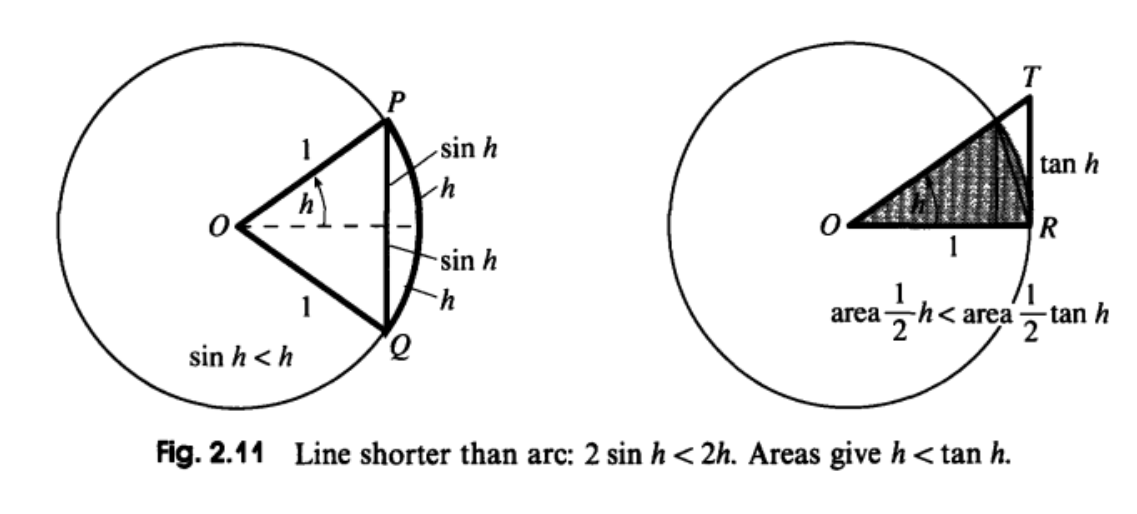
\includegraphics[width=0.9\textwidth]{33pic.png}
\end{center}
which produces
\[
\sin(h) < h, \quad h < \tan(h).
\]
\item Tackle cosine limit via the conjugate.
\item Ask them to prove cosine derivative on own using the same idea and 
\[
\cos(x+h) = \cos(x)\cos(h) - \sin(x)\sin(h).
\]
\end{itemize}
\item Other 4, get from quotient rule connecting to sine and cosine.
\item Note $x$ must be in term of radians here, degrees differ in result by constant.
\item 2 important limits to know.
\end{enumerate}


%%%%%%%%%%%%%%%%%%%%%%%%%%%%%%%%%%%%%%%

%%%%%%%%%%%%%%%%%%%%%%%%%%%%%%%%%%%%%%%
\item Theorem: Derivative of all the trig functions ($\cos x$ is in homework 20, find others by yourself). Show these except cosine via quotient rule.
$$
\frac{d}{dx} \sin(x) = \cos(x), \quad
\frac{d}{dx} \cos(x) = -\sin(x), \quad
\frac{d}{dx} \tan(x) = \sec^2(x)
$$
$$
\frac{d}{dx} \csc(x) = -\csc(x)\cot(x), \quad
\frac{d}{dx} \sec(x) = \sec(x)\tan(x), \quad
\frac{d}{dx} \cot(x) = -\csc^2(x)
$$

%%%%%%%%%%%%%%%%%%%%%%%%%%%%%%%%%%%%%%%
\item Examples:
\begin{enumerate}
\item $$\frac{d}{dx}\frac{\sec x\sin x}{e^x+\tan x}$$
\item Find the second derivative of $\sec x$, note Pythagorean identities to be applied. Many equivalent answers possible.
\item Find the 99th derivative of $\sin x$
\end{enumerate}

%%%%%%%%%%%%%%%%%%%%%%%%%%%%%%%%%%%%%%%
\item Above limit results can be used in weird ways.
\begin{enumerate}
\item 
$$\lim_{\theta\rightarrow 0} \frac{\sin (7\theta)}{3\theta} = 
\lim_{\theta\rightarrow 0} \frac{\sin (7\theta)}{7\theta}\frac{7\theta}{3\theta} = \frac{7}{3}$$
\item Find 
$$\lim_{\theta\rightarrow 0} \frac{\sin(4x)}{\sin(6x)} = \frac{2}{3}$$
\item Mention limit law use and substitution ideas here.
\end{enumerate}
\end{enumerate}


%%%%%%%%%%%%%%%%%%%%%%%%%%%%%%%%%%%%%%%
%%%%%%%%%%%%%%%%%%%%%%%%%%%%%%%%%%%%%%%
\subsection{3.4 The chain rule}

\begin{enumerate}

%%%%%%%%%%%%%%%%%%%%%%%%%%%%%%%%%%%%%%%
\item Take stock: Goal is to diff any function f(x) by...
\begin{enumerate}
\item growing a list of basic functions (trig is next, really sine and cosine are only new ones)
\item combining functions in various ways, new combination here is function composition
\item Short review of function composition
\end{enumerate}

%%%%%%%%%%%%%%%%%%%%%%%%%%%%%%%%%%%%%%%
\item Composition of rates of change
\begin{enumerate}
\item A cheetah is 10x as fast as me. I am 2x as fast as my chicken. How much faster is the cheetah than my chicken? 20x as fast.
\item Example of temperature of La Crosse, temperature in the room, temperature in my storage case.
\item Explanation of chain idea: change in daytime light - changes - temperature - changes - growth of apple tree - changes - size of apple - changes - size of worm population
\item Back to classic function composition diagram. Rate of change in $f\circ g$ at $x$ is the same as ROC of $g$ at $x$ times ROC of $f$ at $g(x)$.
\end{enumerate}

%%%%%%%%%%%%%%%%%%%%%%%%%%%%%%%%%%%%%%%
\item Theorem: Chain rule, for $f$ and $g$ differentiable, $f\circ g$ is also differentiable and
$$
\frac{d}{dx} f(g(x)) = f'(g(x))g'(x)
$$
\begin{enumerate}
\item Proof idea:
\[
\frac{d}{dx} f(g(x)) = \lim_{h \rightarrow 0} \frac{f(g(x+h)) - f(g(x))}{h} = \lim_{h \rightarrow 0} \frac{f(g(x+h)) - f(g(x))}{g(x+h)-g(x)}\frac{g(x+h)-g(x)}{h}
\]
then change of variable and done. See text for technical details.
\item Leibniz notation is convenient.
$$
\frac{dy}{dx} = \frac{dy}{du} \frac{du}{dx}.
$$
\end{enumerate}

%%%%%%%%%%%%%%%%%%%%%%%%
\item Examples:
\begin{enumerate}
\item $(x^2+2x+3)^100$
\item $\tan^3(\sin(x)+1)$
\item $2^x = e^{2\ln(x)}$ leading towards below.
\item Challenge is identifying $f$ and $g$ for composition $f(g(x))$.
\end{enumerate}

%%%%%%%%%%%%%%%%%%%%%%%%%%%%%%%%%%%%%%%
\item This is a versatile new technique. Quotient rule revisited:
$$
\frac{d}{dx} \frac{f(x)}{g(x)} = \frac{d}{dx} f(x)(g(x))^{-1}
$$


%%%%%%%%%%%%%%%%%%%%%%%%%%%%%%%%%%%%%%%
\item General exponential functions 
\begin{enumerate}
\item $2^x = e^{\ln(2)x}$, now differentiate via the chain rule.
\item Theorem:
$$
\frac{d}{dx}a^x = a^x\ln (a)
$$
\item Example: $2^{3^{x^2}}$
\end{enumerate}
\end{enumerate}


%%%%%%%%%%%%%%%%%%%%%%%%%%%%%%%%%%%%%%%
%%%%%%%%%%%%%%%%%%%%%%%%%%%%%%%%%%%%%%%
\subsection{3.5 Implicit differentiation}
\begin{enumerate}

%%%%%%%%%%%%%%%%%%%%%%%%%%%%%%%%%%%%%%%
\item What remains? Extend the chain rule to further our reach.
\begin{enumerate}
\item Inverse functions (log for exp, inv trig, others), next section
\item Curves which are not functions (circle, trajectories, others), this section, tangent lines should still make sense
\end{enumerate}

%%%%%%%%%%%%%%%%%%%%%%%%%%%%%5
\item Example: Find the equation of the tangent line to $x^2+y^2=1$ at point $(1/\sqrt{2}, 1/\sqrt{2})$.
\begin{enumerate}
\item Check that point is actually on the curve. Need $dy/dx$ at this point then done.
\item Assume $y = y(x)$ locally to this point, apply chain rule
\item Note, could have solved for y first in this case, try on own.
\end{enumerate}

%%%%%%%%%%%%%%%%%%%%%%%%%%%%%%%%5
\item Example: Folium of Descartes
\begin{enumerate}
\item $x^3+y^3=6xy$, not a function, cannot solve for $y$
\item Wiki page story, history of calculus
\item Find tangent line at (3,3). Horizontal tangents?
\end{enumerate}

%%%%%%%%%%%%%%%%%%%%%%%%%%%%%%%%%
\item Power rule revisited
\begin{enumerate}
\item Can extend the power rule to rational exponents.
\item $y = x^p/q$ gives $y^q = x^p$, diff both sides and solve.
\item What about irrational powers?
\end{enumerate}

%%%%%%%%%%%%%%%%%%%%%%%%%%%%%%%%%
\item Inverse functions:
\begin{enumerate}
%%%%%%%%%%%%%%%%%%%%%%%%
\item Recall: Inverse function idea
\begin{itemize}
\item General case
\item Simple example: $f(x)=x^2$ and $f^{-1}(x)=\sqrt{x}$. Graph together. Domain and range swap. 
\item Desmos graphs
\end{itemize}

%%%%%%%%%%%%%%%%%%%%%%%5
\item Differentiating inverse functions
\begin{itemize}
\item $f(x) = sqrt(x)$ derivative connected to $f^{-1}(x)=x^2$. Refer to the graph.
\item General case via implicit differentiation: $d/dx f^{-1}(x) = 1/f'(f^{-1}(x))$
\item Note how graph tangent line slope changes when reflected.
\end{itemize}

\end{enumerate}

%%%%%%%%%%%%%%%%%%%%%%%%%%%%%%%%%%%%%%%
\item Derivatives of inverse trigonometric functions
\begin{enumerate}
\item Example: Inverse sine
\begin{itemize}
\item Review of inverse sine (hint at other trig functions, main 4 most important)
\item Restricted sine is invertible.
\item Use implicit differentiation to compute. Check that agrees with previous general inverse function formula. Key is to use a right triangle to eliminate $y$.
\item Key is domain restriction, make sure to write down.
\end{itemize}
\item Domain restrictions for main 4 trig functions.
\begin{itemize}
\item $\arcsin(x), \quad -\frac{\pi}{2} \leq x \leq \frac{\pi}{2}$
\item $\arccos(x), \quad 0 \leq x \leq \pi$
\item $\arctan(x), \quad -\frac{\pi}{2} < x < \frac{\pi}{2}$
\item $\text{arcsec}(x), \quad 0 \leq x \leq \pi$
\end{itemize}
\item 4 derivative formulas. Remember these.
\begin{align*}
\frac{d}{dx} \arcsin(x) &= \frac{1}{\sqrt{1-x^2}}, \quad -1 \leq x \leq 1 \\
\frac{d}{dx} \arccos(x) &= \frac{-1}{\sqrt{1-x^2}}, \quad -1 \leq x \leq 1 \\
\frac{d}{dx} \arctan(x) &= \frac{1}{1+x^2} \\
\frac{d}{dx} \text{arcsec}(x) &= \frac{1}{x\sqrt{x^2-1}}
\end{align*}
\item Example: Use two methods to find the derivative ((students) chain rule, (me) draw triangle and simplify as algebraic expression).
$$
y = \sin(\cos^{-1} x)
$$
\end{enumerate}

\end{enumerate}


%%%%%%%%%%%%%%%%%%%%%%%%%%%%%%%%%%%%%%%
%%%%%%%%%%%%%%%%%%%%%%%%%%%%%%%%%%%%%%%
\subsection{3.6 Derivative of logarithmic functions}
\begin{enumerate}

%%%%%%%%%%%%%%%%%%%%%%%%%%%%%%%%
\item Review of logs:
\begin{enumerate}
\item Definition, keep track of domain and range
\item Log properties
\item Historic motivational interestingness: \url{https://en.wikipedia.org/wiki/History_of_logarithms}
\end{enumerate}

%%%%%%%%%%%%%%%%%%%%%%%%%%%%%%%%%%%%%%%
\item Derivatives of logarithms:
\begin{enumerate}
\item Already can differentiate exponentials. Use implicit differentitation to get at it.
\item Result:
$$
\frac{d}{dx}(\ln x) = \frac{1}{x}
$$
and
$$
\frac{d}{dx}(\log_a x) = \frac{1}{x\ln a}
$$

%%%%%%%%%%%%%%%%%%%%%%%%%%5
\item Examples:
\begin{enumerate}
\item $\frac{d}{dx} (\ln (x^2 e^x)/(x+1))$, leverage log props, can introduce logs when needed, just remove later, see below.
\item Theorem: $\frac{d}{dx}(\ln |x|) = \frac{1}{x}$, force the domains to match, graph in desmos
\end{enumerate}
\end{enumerate}

%%%%%%%%%%%%%%%%%%%%%%%%%%%%%%%%%%%%%%%
\item Logarithmic differentiation: Introduce logs to leverage sweet properties.
\begin{enumerate}
\item Example: $y = x^x$, then $y'=?$ (no such rule)
\item Example: $y = \frac{(x^2+1)(x+3)^{1/2}}{x-1}$, then $y'=?$ (quotient, product, chain rule madness)
\item Summary of steps: 
\begin{enumerate}
\item  Identify the situation (lots of multiplication, quotient, and powers)
\item Take log on both sides (if possible) and simplify using the log properties.
\item Differentiate implicitly with respect $x$
\item Solve for $y'$
\item What if $y=f(x)<0$ for some $x$? Use absolute value.
$$
|y|=|f(x)|, \quad \ln(|y|)=\ln(|f(x)|), \quad \frac{1}{y}\frac{dy}{dx} = \frac{1}{f(x)}f'(x), \quad \frac{dy}{dx}=\dots 
$$
\end{enumerate}
\item Example: Finally, the full power rule: $y = x^n$, $n$ any real number, log differentiation.
\end{enumerate}


%%%%%%%%%%%%%%%%%%%%%%%%%%%%%%%%%%%%%%%
\item Important results to know:
\begin{enumerate}
\item Theorem:
$$
\lim_{x\rightarrow 0} (1+x)^{1/x} = e
$$
Reason: $f(x)=\ln(x)$, then $f'(x)=\frac{1}{x}$ and $f'(1)=1$. So,
$$
1=f'(1)=\lim_{h\rightarrow 0} \frac{1}{h}\ln(1+h)=\lim_{h\rightarrow 0} \frac{\ln(1+h)}{h}=\lim_{h\rightarrow 0} \ln((1+h)^{1/h})
$$
Then, because exponential functions are continuous,
$$
\lim_{x\rightarrow 0}\ln(1+x)^{1/x} = 1 \quad \Rightarrow \quad e=e^1=e^{\lim_{x\rightarrow 0}\ln(1+x)^{1/x}} = \lim_{x\rightarrow 0} (e^{\ln(1+x)^{1/x}})=\lim_{x\rightarrow 0} (1+x)^{1/x}
$$
\item Corollary: Take $n=\frac{1}{x}$ above,
$$
e=\lim_{n\rightarrow \infty}(1+\frac{1}{n})^n \quad \text{(holy compound interest Batman!)}
$$
\item Continuous compounded interest: PERT all ova the place.
$$
\lim_{n\rightarrow \infty}P(1+\frac{r}{n})^{nt}  = Pe^{rt}
$$
\item Wikipedia continuous growth
\item Note, this leans on the previous limit
\[
\lim_{h \rightarrow 0} \frac{e^h-1}{h} = 1
\]
\end{enumerate}
\end{enumerate}


%%%%%%%%%%%%%%%%%%%%%%%%%%%%%%%%%%%%%%%
%%%%%%%%%%%%%%%%%%%%%%%%%%%%%%%%%%%%%%%
\subsection{3.8 Exponential growth and decay}
\begin{enumerate}


%%%%%%%%%%%%%%%%%%%%%%%%%%%%%%%%%%%%%%%
\item Differential equations: Translation of change into calculus  \\
 See the many examples:
\begin{enumerate}
\item \url{https://en.wikipedia.org/wiki/Differential_equation}
\item \url{https://people.maths.ox.ac.uk/trefethen/pdectb.html}
\item Pixar research, Frozen video demo
\item Def: A differential equation is an equation involving derivatives where the unknown is a \emph{function}. (analogous to algebraic equations)
\end{enumerate}

%%%%%%%%%%%%%%%%%%%%%%%%%%
\item DEs and Exponential growth: Population grows at rate proportional to size. 
\begin{enumerate}
\item $\frac{dy}{dx} = r y$, $r$ a postitive constant, $y(0)$ initial condition.
\item Example: $r = 1, y(0) = 10$. Graph and interpret. $r = 2, -3$?
\item General solution $y = y(0)e^{rt}$
\item Trouble is, don't usually know $r$. Need to find this from data.
\item La Cross population growth. Find population now and 10 years ago. Project population in 10 year. Plot result in desmos. Google real trends.
\item Issue: Exponential growth is unrealistic long term. Can modify rule.
\end{enumerate}

%%%%%%%%%%%%%%%%%%%%%%%%%%%%
\item Improved population growth. Assume a carry capacity $L$.
\begin{enumerate}
\item $y << L$ increase fast then slow down, $y >> L$ decrease fast then slow down, $y \approx L$ little change, $y \approx 0$ little change.
\item Harder to solve by hand, but this one is doable, often not possible.
\item Approximate with slope field. Google dfield.
\item Google logistic growth.
\end{enumerate}
\end{enumerate}


%%%%%%%%%%%%%%%%%%%%%%%%%%%%%%%%%%%%%%%
%%%%%%%%%%%%%%%%%%%%%%%%%%%%%%%%%%%%%%%
\subsection{3.9 Related rates}
\begin{enumerate}

%%%%%%%%%%%%%%%%%%%%%%%%%%%%%%%%
\item Key idea: Which rates are related?
\begin{itemize}
\item Snowball melting youtube. List all things changing. Which are connected?
\item \url{https://www.youtube.com/watch?v=LNEBZ8ekU18}
\item Volume of sphere formula. Time as variable.
\item Example: Suppose snowball is melting at $5 cm^3$ per minute. How fast is the diameter shrinking when $r=4cm$?
\item Steps: Picture, assign variables, rates as derivatives comb with data, equation relating all vars, implicit differentiation.
\end{itemize}

%%%%%%%%%%%%%%%%%%%%%%%%%%%%%%%%%%%%%%%
\item Example: A ladder 10 ft long is sliding against a vertical wall. If the bottom of the ladder slides away from the wall at a rate of 1ft/s, how fast is the top of the ladder sliding down the wall when the bottom of the ladder is 6ft from the way?
\begin{enumerate}
\item Drawing picture is key, Pythagorean theorem is connection.
\item What is the changing rate of $\theta$?
\end{enumerate}

%%%%%%%%%%%%%%%%%%%%%%%%%
\item Example: Boat pulled to dock by rope 1 ft above the bow of boat. If the rope is pulled at 1 ft / sec, how fast is the boat approaching the dock when 8 ft from doc?


%%%%%%%%%%%%%%%%%%%%%%%%%%%%%%%%%%%%%%%
\item Global positioning system story of related rates. Student at MIT. \url{http://www.pcworld.com/article/2000276/a-brief-history-of-gps.html}
\end{enumerate}

%%%%%%%%%%%%%%%%%%%%%%%%%%%%%%%%%%%%%%%
%%%%%%%%%%%%%%%%%%%%%%%%%%%%%%%%%%%%%%%
\subsection{3.10 Linear approximations and differentials }
\begin{enumerate}

%%%%%%%%%%%%%%%%%%%%%%%%%%%%%%%%%%%%%%%
\item Motivation and idea:
\begin{enumerate}
\item Practical questions: What is $\sqrt{4.1}$, $\sin(46^\circ)$?
\item Idea: Use the value of a function around a known $f(a)$ in a smart way.
\item Think of
$$
f'(a)=\lim_{x\rightarrow a}\frac{f(x)-f(a)}{x-a}
$$
When $x$ is close to $a$ they basically satisfies the relationship.
\end{enumerate}

%%%%%%%%%%%%%%%%%%%%%%%%%%%%%%%%%%%%%%%
\item Linear approximation: the linear (tangent line) approximation of $f$ at $a$ is 
$$
L(x) = f(a)+f'(a)(x-a)
$$
Also known as the linearization of $f$ at $a$. Compare to limit of difference quotient above.
\begin{enumerate}
\item Idea: $f(x)$ is ``locally" a line (around $a$), draw picture of $f$ and $L$
\item This is an approximation and may not be accurate at all
\begin{itemize}
\item depending on the original shape
\item depending on how close your $x$ is to $a$
\end{itemize}
\end{enumerate}

%%%%%%%%%%%%%%%%%%%%%%%%%%%%%%%%%%%%%%%
\item {\bf Examples:} Find the linearization of $\sqrt{x}$ at $4$
\begin{enumerate}
\item Use it to approximate $\sqrt{4.1}$, $\sqrt{4.5}$, $\sqrt{6}$ and compare to the real value.
\item Find $\sin(44^\circ)$, do the same thing.
\item In physics, $\sin x\approx x$ when $x$ is small. This is linearization.
\end{enumerate}

%%%%%%%%%%%%%%%%%%%%%%%%%%%%%%%%%%%%%%%
\item Differentials: 
$$
dy = f'(x) dx
$$
\begin{enumerate}
\item What is this? Reminds of $\frac{dy}{dx}=f'(x)$. What if treat as a ration?
\item Find the differential of $x^2$ at $x =2$. Pick different $dx$ and graph.
\item Difference between $dy$ and $\triangle y$. Actually, $dy=\delta L$.
\item This is close to the original conceptualization of calculus.
\end{enumerate}

%%%%%%%%%%%%%%%%%%%%%%%%%%%%%%%%%%%%%%%
\item {\bf Example:}  A sphere was measured and its radius was found to be 45 inches with a possible error of no more that 0.01 inches.  
What is the maximum possible error in the volume if we use this value of the radius?
\[
V = \frac{4}{3}\pi r^3 \quad \Rightarrow \quad \Delta V \approx dV = 4\pi r^2 dr
\]

%%%%%%%%%%%%%%%%%%%%%%%%%%%%%%%%%%%%%%%
\item Can we replace $f(x)$ locally by a quadratic equation?
\begin{enumerate}
\item Doable? (Yes, need first and second derivatives to match)
\item More work? (Yes)
\item Better accuracy? (Yes)
\item Any polynomial? (Taylor polynomial, calculus 2)
\item Why bother replacing functions with polynomials? (Biggest take-away of the section)
\begin{itemize}
\item Approximation of hard calculations
\item Polynomials are nicer functions than anything else, so live in a better place.
\end{itemize}
\item Can we use things other than polynomials? Sure thing (Fourier series) for periodic functions (light, sound, universe of waves).
\end{enumerate}
\end{enumerate}


%%%%%%%%%%%%%%%%%%%%%%%%%%%%%%%%%%%%%%%
%%%%%%%%%%%%%%%%%%%%%%%%%%%%%%%%%%%%%%%
\subsection{3.11 Hyperbolic functions}
\begin{enumerate}

%%%%%%%%%%%%%%%%%%%%%%%%%%%%%%%%%%%%%%%
\item Motivation:  
\begin{enumerate} 
\item Think about a heavy flexible cable suspended between two points at the same height (the golden gate bridge, telephone cable). This is called a catenary. What is that curve? Not quite a parabola.
\url{https://www.google.com/search?q=catenaries&espv=2&biw=1680&bih=921&tbm=isch&tbo=u&source=univ&sa=X&ved=0ahUKEwj5552K2ejKAhVCFR4KHRoADp8QsAQIQw#tbm=isch&q=catenary&imgrc=ES8GEHgRx3OpXM%3A}
$$
\frac{e^x+e^{-x}}{2}
$$
\item What's the derivative?
\end{enumerate}

%%%%%%%%%%%%%%%%%%%%%%%%%%%%%%%%%%%%%%%
\item The family of hyperbolic functions, such parallels with regular trigonomety here.
$$
\sinh x  = \frac{e^x-e^{-x}}{2},\quad\cosh x  = \frac{e^x+e^{-x}}{2}
$$
\begin{enumerate}
\item Regular division and such gives the rest. $\tanh(x)=, \dots$.
\item Just as the points $(\cos(t), \sin(t))$ form a circle with a unit radius, the points $(\cosh(t), \sinh(t))$ form the right half of the equilateral hyperbola $x^2-y^2=1$. 
\item For some applications, this is the correct geometry (special relativity).
\end{enumerate}

%%%%%%%%%%%%%%%%%%%%%%%%%%%%%%%%%%%%%%%
\item Hyperbolic identities:
\begin{enumerate}
\item Odd, even:
$$
\sinh(-x) = -\sinh(x),\quad \cosh(-x) = \cosh(x)
$$
\item The "Pythagorean" identities:
$$
\cosh^2 x-\sinh^2 x = 1,\quad 1-\tanh^2  = sech^2x
$$
\item The sum formula:
$$
\sinh(x+y) = \sinh(x)\cosh(y)+\cosh(x)\sin(y)
$$
$$
\cosh(x+y) = \cosh(x)\cosh(y)+\sinh(x)\sin(y)
$$
\item Double angle formula:
$$
\sinh(2x) = 2\sinh x\cosh x
$$
\end{enumerate}

%%%%%%%%%%%%%%%%%%%%%%%%%%%%%%%%%%%%%%%
\item Derivatives of hyperbolic functions (show this)
$$
(\sinh x)' = \cosh x
$$

%%%%%%%%%%%%%%%%%%%%%%%%%%%%%%%%%%%%%%%
\item Inversere hyperbolic function (show this, substitution, hidden quadratic)
$$
\sinh^{-1}(x) = \ln (x+\sqrt{x^2+1})
$$

\item What you need to know:
\begin{enumerate}
\item Know they come from application. Be aware.
\item You don't have to memorize anything but the definition of the hyperbolic sine and cosine.
\item Feel free to check the book when you do the homework
\item I may test it as an exercise of derivatives.
\end{enumerate}
\end{enumerate}


%%%%%%%%%%%%%%%%%%%%%%%%%%%%%%%%%%%%%%%
%%%%%%%%%%%%%%%%%%%%%%%%%%%%%%%%%%%%%%%
\section{Chapter 4 Applications of differentiation}

\begin{enumerate}
\item We've seen some applications in Ch3, but the list is long. Sometimes seem more mathy than useful.
\begin{enumerate}
\item \url{https://en.wikipedia.org/wiki/Differential_calculus#Applications_of_derivatives}
\item \url{https://en.wikipedia.org/wiki/Mathematical_optimization}
\end{enumerate}

\item Chapter outline:
\begin{enumerate}
\item Deeper function understanding: Graphing with detail
\item Optimization: Max and min values
\item Theory: MVT
\item Beginnings: Reversing differentiation, called integration
\end{enumerate}
\end{enumerate}

%%%%%%%%%%%%%%%%%%%%%%%%%%%%%%%%%%%%%%%
%%%%%%%%%%%%%%%%%%%%%%%%%%%%%%%%%%%%%%%
\subsection{4.1 Maximum and minimum values}

%%%%%%%%%%%%%%%%%%%%%%%%%%%%%%%%%%%%%%%
\begin{enumerate}
\item Extreme values of functions: Local min and max, absolute min and max.
\begin{enumerate}
\item Main application: Optimization, largest, cheapest, fastest.
\item Def of abs min / max, local min / max
\item Eg. Local min if $f(c) <= f(x)$ for all $x$ near $c$
\item Draw picture to illustrate.
\item Possible locations: Zero derivatives, corners, discontinuities, endpoints, inflection pts
\end{enumerate}

%%%%%%%%%%%%%%%%%%%%%%%%%%%%%%%%%%%%%%%
\item Extreme value theorem (EVT)
\begin{enumerate}
\item How to ensure EVs happen? Avoid the bad scenarios: holes, asymptotes.
\item EVT: If $f(x)$ is continuous on closed interval $[a,b]$, then $f(x)$ must attain EV on $[a,b]$.
\item Note, does not say where it is or how to find, just that it exists.
\end{enumerate}

%%%%%%%%%%%%%%%%%%%%%%%%%%%%%%%%%%%%%5
\item How to find extreme values?
\begin{enumerate}
\item Must occur at a critical number.
\item Cases for critical numbers: Endpoints, stationary points, singular points.
\end{enumerate}


%%%%%%%%%%%%%%%%%%%%%%%%%%%%%%%%%%%%%%%
\item Example: Find the absolute max and min by checking the critical numbers. Use Desmos to check.
\begin{enumerate}
\item $f(x) = x^3+x^2-x$ on $[-2,2]$. 
\item $f(x) = x^{\frac{2}{3}}$, no interval then add open / closed. Change to $x^\frac{1}{3}$
\item $f(x) = x + 2\cos(x)$ on $[0,2\pi]$
\end{enumerate}
\end{enumerate}	



%%%%%%%%%%%%%%%%%%%%%%%%%%%%%%%%%%%%%%%
%%%%%%%%%%%%%%%%%%%%%%%%%%%%%%%%%%%%%%%
\subsection{4.2 The mean value theorem}

\begin{enumerate}

%%%%%%%%%%%%%%%%%%%%%%%%%%%5
\item Big picture of the MVT:
\begin{enumerate}
\item Math theory detour, useful for proofiness rather than application
\item Big picture: Connect IROC and AROC, no limits
\item Most used calculus result in math world
\end{enumerate}

%%%%%%%%%%%%%%%%%%%%%%%%%%%%%%%%%%%%%%%
\item Rolle's Theorem: Let function $f(x)$ be continuous on $[a,b]$ and differentiable on $(a,b)$ with $f(a)=f(b)$. Then there's a number $c$ in $(a,b)$ such that $f'(c) = 0$. 
\begin{enumerate}
\item Ask to draw picture and see why true.
\item More than one $c$ possible.
\item Why is closed interval important? Diff? $f(a)=f(b)$?
\end{enumerate}

%%%%%%%%%%%%%%%%%%%%%%%%%%%%%%%%%%%%%%%
\item Example: Show that $x^3+x-1 = 0$ has only one real solution.
\begin{enumerate}
\item Using IVT on $[0,1]$ to show existence.
\item What if had 2 zeros on $(0,1)$, $f(a)=f(b)=0$? Then Rolle's theorem says there is $c$ in $(a,b)$ such that $f'(0)=0$. But, $f'(x)=3x^2+1$. So, can only have 1 zero.
\end{enumerate}

%%%%%%%%%%%%%%%%%%%%%%%%%%%%%%%%%%%%%%%
\item Mean Value Theorem: Let function $f(x)$ be continuous on $[a,b]$ and differentiable on $(a,b)$. Then there's a number $c$ in $(a,b)$ such that 
\[
f'(c) = \frac{f(b)-f(a)}{b-a}.
\] 
\begin{enumerate}
\item Ask to draw picture and see why true.
\item More than one $c$ possible.
\item Why is closed interval important? Diff? $f(a)=f(b)$?
\item Average rate of change equals inst rat of change.
\item When you are driving, there'll always be a moment that your instantaneous velocity is the same as the average velocity.
\item Suppose you are driving from La Crosse to Madison: 150 mile, 1.5 hours. What should the speeding ticket be written for? 100mile/h
\end{enumerate}

%%%%%%%%%%%%%%%%%%%%%%%%%%%%%%%%%%%%%%%
\item Example: Find an upper bound on difference $\cos(1)-\cos(1.1)$.
\begin{enumerate}
\item Apply MVT via rearrangement. Check hypothesis first.
\item Connected to linearization.
\end{enumerate}

%%%%%%%%%%%%%%%%%%%%%%%%%%%%%%%%%%%%%%%
\item Theorems: The power of MVT
\begin{enumerate}
\item If $f'(x)=0$ on $(a,b)$, then $f$ is constant on $(a,b)$.
\[
0 = f'(x) = (f(x_1)-f(x_2))/(x_1-x_2)
\]
for all $x_1,x_2$ on $(a,b)$, then $f(x1)=f(x2)$.
\item If $f'(x)=g'(x)$ on $(a,b)$, then $f(x)=g(x)+C$ for some constant $C$
\[ 
h(x)=f(x)-g(x) \quad \Rightarrow \quad h'(x)=0
\]
and $h(x)=C$ by above theorem.
\end{enumerate}
\end{enumerate}


%%%%%%%%%%%%%%%%%%%%%%%%%%%%%%%%%%%%%%%
%%%%%%%%%%%%%%%%%%%%%%%%%%%%%%%%%%%%%%%
\subsection{4.3 How derivatives affect the shape of a graph}

%%%%%%%%%%%%%%%%%%%%%%%%%%%%%%%%%%%%%%%
\begin{enumerate}
\item Example
\begin{enumerate}
\item Graph $f(x)$, $f'(x)$ and $f''(x)$ for $f(x) = x^3+x^2-x$
\item How is $f'$ related to $f$, $f''$ to $f'$, $f''$ to $f$?
\item Desmos
\end{enumerate}

%%%%%%%%%%%%%%%%%%%%%%%%%%%%%%%%%%%%%%%
\item First derivative $f'(x)$
\begin{enumerate}
\item {\bf Increasing/decreasing test}
\begin{itemize}
\item If $f'(x) >0$, then $f$ is increasing ($a<b$ gives $f(a)<f(b)$)
\item If $f'(x)<0$, then $f$ is decreasing ($a<b$ gives $f(a)>f(b)$)
\end{itemize}
\item {\bf The first derivative test} Suppose $c$ is a critical number for $f$ (possible local max/min). Let them fill in blank.
\begin{itemize}
\item If $f'(x)$ changes from positive to negative at $c$, then .... $f$ has a local max at $c$.
\item If $f'(x)$ changes from negative to positive at $c$, then .... $f$ has a local min at $c$.
\item If $f'(x)$ does not change sign at $c$, then .... $f$ has no local max or min at $c$.  (called a saddle point)
\end{itemize}
\end{enumerate}

%%%%%%%%%%%%%%%%%%%%%%%%%%%%%%%%%%%%%%%
\item  Example: Draw number line to find inc/dec. Find min/maxs. Draw on own.
\begin{enumerate}
\item $f(x) =3x^4-4x^3-12x^2+5$ 
\item How to graph $f$? Have a pretty good picture. What else can we add for detail? Where are turning points? Zeros?
\end{enumerate}

%%%%%%%%%%%%%%%%%%%%%%%%%%%%%%%%%%%%%%%
\item Second derivative $f''(x)$, above example. Let them fill in blank.
\begin{enumerate}
\item {\bf Concavity test}
\begin{itemize}
\item If ... $f''(x)>0$, then $f$ is  concave up
\item If ... $f''(x)<0$, then $f$ is  concave down
\end{itemize}
\item {\bf The second derivative test: }
\begin{itemize}
\item $f'(c) = 0$, $f''(c) >0$, local min
\item $f'(c)=0$, $f''(c)<0$, local max
\end{itemize}
\item Used to find local max/min, easier than first derivative test.
\item If $f''(x)=0$, it's inconclusive. Why? Think of a graph. This is an inflection point.
\item When can't the second derivative test be used? If $f''$ does not exist (corner)
\end{enumerate}

%%%%%%%%%%%%%%%%%%%%%%%%%%%%%%%%%%%%%%%
\item {\bf Examples:} Graph sketching
\begin{enumerate}
\item Finish above example. Add inflection point.
\item Try on own: $f(x) = x^3-3x^2-9x+4$, .
\end{enumerate}
\end{enumerate}



%%%%%%%%%%%%%%%%%%%%%%%%%%%%%%%%%%%%%%%
%%%%%%%%%%%%%%%%%%%%%%%%%%%%%%%%%%%%%%%
\subsection{4.4 Indeterminate forms and L'Hospital Rule}

\begin{enumerate}
%%%%%%%%%%%%%%%%%%%%%%%%%%%%%%%%%%%%%%%
\item Recall: Indeterminate form, the reason for limits.
\begin{enumerate}
\item Limit of difference quotient. $0/0$ IF. Limit idea invented to handle this problem. 
\item Already have algebraic techniques: $f(x)=x^2, f'(1)=$? $f(x)=\sqrt{x}, f'(1)=$?
\item Our techniques are not enough: $f(x)=\ln(x), f'(1)=$? Used the inverse relation to handle in past. 
\item Key: Indeterminate forms can be ANYTHING. Modify above example to show 2, 200, $\pi$, $\infty$, 0, etc.
\item Types of indeterminate form:
\begin{itemize}
\item Quotient $0/0$
\item Quotient $\infty/\infty$
\item Product $0\cdot \infty$
\item Difference $\infty-\infty$
\item Exponent $0^0, 1^\infty$, $\infty^0$
\item Strategy: Rewrite all as first two quotients.
\end{itemize}
\end{enumerate}

%%%%%%%%%%%%%%%%%%%%%%%%%%%%%%%%%%%%%%%
\item Theorem: (l'Hospital's Rule) If $f$ and $g$ are differentiable around $x=a$, and $\displaystyle\lim_{x\rightarrow a} \frac{f(x)}{g(x)}$ is of indeterminate form $0/0$ or $\infty/\infty$, then
$$
\lim_{x\rightarrow a} \frac{f(x)}{g(x)} = \lim_{x\rightarrow a} \frac{f'(x)}{g'(x)}
$$
if $\displaystyle\lim_{x\rightarrow a} \frac{f'(x)}{g'(x)}$ exists or is $\pm\infty$

\begin{enumerate}
\item Proof idea ($0/0$ IF case): Close to $x=a$, replace $f(x)$ with linearization $f'(a)(x-a)$ (tangent line approximation). Draw graph. Likewise for $g$. Cancel $(x-a)$ factor to get result.
\item Tangent line tells rate to 0 or inf. This is the tug of war.
\item Note: LR works for one sided limits also
\end{enumerate}

%%%%%%%%%%%%%%%%%%%%%%%%%%%%%%%%%%%%%%%
\item Examples: Check on own. Check if LR hypothesis holds first.
\begin{enumerate}
\item $\ds \lim_{x \rightarrow 1} (x^2-1)/(x-1)$
\item $\ds \lim_{x \rightarrow 1} ln(x)/(x-1)$
\item Can get crazy: Which grows faster, $x^{1000}$ or $e^x$? How to tell? Look at the ratio: $\ds \lim_{x\rightarrow \infty} \frac{x^{1000}}{e^x}$
\item Old limits are easier:
$$
\lim_{x\rightarrow 0 } \frac{\sin x}{x} = 1,\quad 
\lim_{h\rightarrow 0} \frac{\sin h}{h} = 2/3,\quad 
\lim_{x\rightarrow 0} \frac{\sin 2x}{\sin 3x} = 2/3
$$
\item Beware of temptation: 
$$\lim_{x\rightarrow \infty} \frac{\sqrt{x^2-1}}{x} = ?$$
\end{enumerate}

%%%%%%%%%%%%%%%%%%%%%%%%%%%%%%%%%%%%%%%
\item Other indeterminate forms: Idea is to always transfer to $0/0$ or $\infty/\infty$ form.
\begin{enumerate}
\item $\ds \lim_{x \rightarrow 0^+} (1/x - 1/(e^x-1))$ (add fractions)
\item $\ds \lim_{x \rightarrow 0} x^x$ (log and exp, then log prop)
\item $\ds \lim_{x \rightarrow inf} (1+1/x)^x$
\item Mention it's super important: indeterminant form is the most common case we want to work on. (derivative, def integral, etc)
\end{enumerate}
\end{enumerate}



%%%%%%%%%%%%%%%%%%%%%%%%%%%%%%%%%%%%%%%
%%%%%%%%%%%%%%%%%%%%%%%%%%%%%%%%%%%%%%%
\subsection{4.5 Summary of curve sketching}
\begin{enumerate}

%%%%%%%%%%%%%%%%%%%%%%%%%%%%%%%%%%%%%%%
\item Guidelines for curve sketching (we've already covered this!):
\begin{enumerate}
\item Find the omain
\item Locate $x$ and $y$ intercepts
\item Does $f$ have symmetry (even or odd)?
\item Asymptotes (horizontal, vertical, oblique)
\item Where is $f$ increasing / decreasing?
\item Find local mins and maxes (critical pts and 1st or 2nd derivative test)
\item Concavity and points of inflection 
\item Put all together to get a fantastic picture
\end{enumerate}

%%%%%%%%%%%%%%%%%%%%%%%%%%%%%%%%%%%%%%%
\item {\bf Examples:}
\begin{enumerate}
\item $f(x) = \frac{1+2x^2}{1-x^2}$ (horizontal and vertical asymptotes)
\item $ g(x) = \frac{-3x^2+2}{x-1}$ (oblique asymptote, need long division)
\end{enumerate}
Read the section and finish the homework!
\end{enumerate}


%%%%%%%%%%%%%%%%%%%%%%%%%%%%%%%%%%%%%%%
%%%%%%%%%%%%%%%%%%%%%%%%%%%%%%%%%%%%%%%
\subsection{4.7 Optimization problmes}

\begin{enumerate}
%%%%%%%%%%%%%%%%%5
\item Idea:
\begin{enumerate}
\item Find min/max of a target function $f(x)$ subject to some sort of constraint ($a \leq x \leq b$).
\item Same as abs min / max problem.
\item Check critical points (stationary, singular, endpoints)
\item Difficulty is translating the problem into math (function, relating variables, etc)
\end{enumerate}

%%%%%%%%%%%%%%%%%%%%%%%%%%%%%%%%%%%%%%%
\item Chicken fence next to dog area:Try on own
\begin{enumerate}
\item 200 ft of fence, on corner of dog fence (10ft and 20ft sides). What is the maximum area enclosed?
\item Generalize to steps as with related rates.
\end{enumerate}

%%%%%%%%%%%%%%%%%%%%%%%%%%%%%%%%%%%%%%%
\item Optimization problem strategy:
\begin{enumerate}
\item Make sure it's an optimization problem (-est, most, least)
\item Draw a picture to help
\item Find the variable $y$ that you want to minimize/maximize, introduce other notation
\item Find the changing variable $x$
\item Write $y = f(x)$ as a function of $x$, eliminate other variables if needed
\item Identify an closed interval for $x$ (why necessary? Extreme Value Theorem)
\item Find the extreme value of $y$
\item Answer the original question in words
\end{enumerate}

%%%%%%%%%%%%%%%%%%%%%%%%%%%%%%%%%%%%%%%
\item {\bf Examples:}
\begin{enumerate}
\item A cylindrical can is required to hold $1$ liter of oil. Design the can to minimize the use of material. 
\[
S = 2\pi r^2 + 2\pi r h, \text{ (eliminate $h$, can also use implicit diff)}
\]
\item Find the point on the curve $ y = 2x-1$ closest to the point (3, 2). 
\[
d = \sqrt{(x-2)^2+(y-2)^2}, \text{ (can eliminate or implicit diff)}
\]
\item What's the area of the biggest rectangle that can be inscribed inside a unit circle?
\[
A = 2xy = 2x\sqrt{1-x^2}
\]
\end{enumerate}
\item So many applications here, especially in business.
\begin{itemize}
\item Wiki page
\item UWL journal ug research paper
\end{itemize}
\end{enumerate}


%%%%%%%%%%%%%%%%%%%%%%%%%%%%%%%%%%%%%%%
%%%%%%%%%%%%%%%%%%%%%%%%%%%%%%%%%%%%%%%
\subsection{4.8 Newton's method}

\begin{enumerate}
%%%%%%%%%%%%%%%%%%%%%%%%%%%%%%%%%%%%%%%
\item {\bf Motivating Example} Solve $x^3-3x+1 = 0$
\begin{itemize}
\item Pick place to start: $x_0 = 0$
\item Find the linearization at $(x_0, y_0)$
\item Follow linearization to get zero which approximates $f$'s zero.
\item Show Desmos right away
\item Write down the formula
$$
x_{n+1} = x_n -\frac{f(x_n)}{f'(x_n)}
$$
\item Do the iteration by hand
\item Do $x_0 = 7$, $4$.
\end{itemize}

%%%%%%%%%%%%%%%%%%%%%%%%%%%%%%%%%%%%%%%
\item Idea of Newton's method
\begin{enumerate}
\item Again, replace $f$ by linearization (calculus), sweet move.
\item Does it always work? What could go wrong? We need more than just a formula.
\begin{enumerate}
\item Could be no root at all (IVT to check existence)
\item Could hit zero derivative, shoot to infinity (zero division)
\item Find wrong root. 
\item Even though the formula stays the same, the result depends on the initial value $x_1$
\item Slows down at roots with multiplicity.
\item Sometimes it just doesn't work (MVT, diverges to infinity)
$$
x^{1/3}=0, \quad x_1 = 1.
$$
\item Under the right assumptions (continuous and differentiable around the root, choose $x_1$ close enough), can prove Newton's method is fast and effective.
\end{enumerate}
\end{enumerate}

%%%%%%%%%%%%%%%%%%%%%%%%%%%%%%%%%%%%%%%
\item Find the solution of $\cos x = x$ using the Newton's method
\begin{enumerate}
\item Draw a picture to see how many solutions are there
\item Find the iteration method
\item For which initial value does it fail
\item Assign the initial value 
\item Compute the result
\item Mention fixed point methods if interested $x_n = \cos(x_{n-1})$
\end{enumerate}

%%%%%%%%%%%%%%%%%%%%%%%%%%%%%%%%%%%%%%%
\item Mind-blowing awesomeness:
\begin{enumerate}
\item \url{http://octave-online.net/}
\item $\sqrt{2}$ via $x^2=2$.
\item $\pi$ via $\sin(x)=0$ fast, $\cos(x)=1$ slow. Why? Multiplicity of root.
\item R pseudocode:
\begin{verbatim}
# newton's method
options(digits=16)

f <- function(x){x^2-2}
fp <- function(x){2*x}

x <- 1
for (i in c(1:10)){
  x <- x - f(x)/fp(x)
  print(x)
}
\end{verbatim}
\end{enumerate}

%%%%%%%%%%%%%%%%%%%%%%%%%%%%%%%%%%%%%%%\item More
\begin{enumerate}
\item How to improve on Newton? Taylor series to higher order
\item Fractals and complex numbers
\begin{itemize}
\item Zoomin: \url{https://www.youtube.com/watch?v=0jGaio87u3A}
\item Applications: \url{https://en.wikipedia.org/wiki/Fractal#Applications_in_technology}
\item Nature: \url{https://www.google.com/search?q=fractal+nature&espv=2&biw=1309&bih=781&tbm=isch&tbo=u&source=univ&sa=X&ved=0ahUKEwjS677XsIbMAhUMMSYKHSwkBC0QsAQIGw}
\end{itemize}
\end{enumerate}
\end{enumerate}


%%%%%%%%%%%%%%%%%%%%%%%%%%%%%%%%%%%%%%%
%%%%%%%%%%%%%%%%%%%%%%%%%%%%%%%%%%%%%%%
\subsection{4.9 Anti-derivatives}
\begin{enumerate}

%%%%%%%%%%%%%%%%%%%%%%%%%%%%%%%%%%%%%%%
\item Motivation: Goal is to reverse differentiation. Key here is lack of uniqueness.
\begin{enumerate}
\item Many physical laws quantify change, but computing the underlying quantities is most interesting.
\item Saw this already with DEs for exponential growth.
\item Conservation law.
\item Free fall $a(t) = 9.8 m/s^2$, can get velocity and distance. Free fall with drag $a(t) = 9.8 - kv$ (gravity const - drag).
\item Kepler's laws of planetary motion spurred Newton to work on Calculus and support theory of physics.
\item Any physical (or other) law.
\end{enumerate}

%%%%%%%%%%%%%%%%%%%%%%%%%%%%%%%%%%%%%%%
\item Def: $f(x)$ is an antiderivative of $f(x)$ on interval $I$ if $f'(x) = f(x)$ for all $x$ in $I$
\begin{enumerate}
\item Example: $2x$ has antiderivative $x^2$
\item Note, not unique here. Any $f(x)+C$ works for $C$ an arbitrary constant. Graph multiple antiderivatives.
\item Think of derivative as an operator we aim to reverse.
\end{enumerate}

%%%%%%%%%%%%%%%%%%%%%%%%%%%%%%%%%%%%%%%
\item Def: The collection of all antiderivatives of $f(x)$ is denoted $\int f(x) ~dx$. That is, $\int f(x) ~dx=F(x)+C$ where $F(x)$ is any antiderivative and $C$ an arbitrary constant.
\begin{enumerate}
\item New idea to capture all reverse derivatives.
\item Example: $\int 2x ~dx$
\item Will explain notation in Chapter 5.
\end{enumerate}


%%%%%%%%%%%%%%%%%%%%%%%%%%%%%%%%%%%%%%%
\item Theorem: Properties of the indefinite integral come from differentiation. They are easily checked through that lens.
\begin{enumerate}
\item $\ds \int cf(x) ~dx = c\int f(x) ~dx$
\item $\ds \int f(x) + g(x) ~dx = \int f(x) ~dx + \int g(x)~ dx$
\item This allows us to treat $\int ~dx$ as an operator much like $\frac{d}{dx}$.
\end{enumerate}

%%%%%%%%%%%%%%%%%%%%%%%%%%%%%%%%%%%%%%%
\item Examples:
\begin{enumerate}
\item Integration rules (no need to memorize, just reasoning): $k, x^n, \frac{1}{x}, \sin(x), \cos(x), \sec^2(x), \csc^2(x)$
\item $\sec(x)\tan(x), \csc(x)\cot(x), e^x, e^{kx}, a^x, \frac{1}{1+x^2}$
\item $\int( 1+\sin(x)+4x^2+2^x) ~dx$ 
\item Not always easy: $2x\cos(x^2)$, $\tan(x)$, $xe^x$
\item Find $f(x)$ such that $f''(x) = x^2$ and $f(3)=1$, $f'(4)=1$.
\end{enumerate}
\end{enumerate}


%%%%%%%%%%%%%%%%%%%%%%%%%%%%%%%%%%%%%%%
%%%%%%%%%%%%%%%%%%%%%%%%%%%%%%%%%%%%%%%
\section{Chapter 5}

\begin{enumerate}
\item Second paradox of calculus: Area under the curve
\begin{enumerate}
\item Area under the curve.
\item Why bother?
\begin{itemize}
\item Lots of applications, anything involving accumulation.
\item Probs to chance, velocity to disp, force to work, Calc 2 etc
\end{itemize}
\item Approach? Mirror tangent line
\begin{itemize}
\item Approximation, limiting process, indet form. Again limit is key.
\item Deep connection to derivative.
\item FTOC: Newton connected IROC to AUC, Leibnitz did AUC to IROC
\end{itemize}
\end{enumerate}

\item Chapter outline:
\begin{enumerate}
\item Area under curve.
\item FTOC
\item Basic integration techniques.
\end{enumerate}
\end{enumerate}

%%%%%%%%%%%%%%%%%%%%%%%%%%%%%%%%%%%%%%%
\subsection{5.1 Areas and distances}

\begin{enumerate}

%%%%%%%%%%%%%%%%%%%%%%%%%%%%%%%%%%%%%%%
\item Motivation: Classic problem of physics: $d=rt$
\begin{enumerate}
\item $s=s(t)$, we know $\frac{ds}{dt} = v$. What about the reverse connection? Our car knows...maybe.
\item Constant velocity case, 60mph for 4 hrs. Graph. Distance is AUC.
\item Changing velocity, can approximate velocity and approximate AUC. Smaller subintervals the better. See the tug of war.
\item Think of summing up velocity to get distance.
\end{enumerate}

%%%%%%%%%%%%%%%%%%%%%%%%%%%%%%%%%%%%%%%
\item Example: Approximating AUC
\begin{enumerate}
\item $f(x)=x^2+1$ on $[0,2]$
\item Approximate by simple shapes. 4 rectangles of equal base.
\item Lots of ways to choose sample point: Left, right, midpoint.
\item Desmos and Riemann sum. More rectangels. Take the limit to get the whole way. Trouble is how to formalize this process.
\end{enumerate} 

%%%%%%%%%%%%%%%%%%%%%%%%%%%%%%%%%%%%%%%
\item Example: Approximating AUC
\begin{enumerate}
\item $f(x)=x^2+1$ on $[0,2]$
\item Chop into equal width subintervals. $n$ total.
\item Choose right endpoint as sample point $x_i$. Other options are left and midpoint.
\item Simplify Riemann sum via $f$.
\item Need special summation formulas involving $i, i^2, i^3$, more?
\begin{itemize}
\item Def of summation notation, simple example.
\item Theorem: Special summation formulas for $i, i^2, i^3$.
\item Theorem: Properties of summation ($ca_i$, $(a_i+b_i)$)
\end{itemize}
\item Finish previous example.
\end{enumerate}

%%%%%%%%%%%%%%%%%%%%%%%%%%%%%%%%%%%%%%%
\item Def: AUC as limit of Riemann sum
\begin{enumerate}
\item Draw general picture.
\item Clarify notation, $[a,b], f(x), x_i, x_i^*, \Delta x$.
\item Challenge, need to simplify the summation to compute limit. Usually hard.
\end{enumerate}

%%%%%%%%%%%%%%%%%%%%%%%%%%%%%%%
\item Example: Try on own. Find AUC of $f(x)=-2x+6$ on $[0,4]$. Check via geometry. Note the signed AUC.

%%%%%%%%%%%%%%%%%%%%%%%%%%
\item Area thru history: Archimedes and quadrature of parabola, volume of sphere, Cavaliri principle

\end{enumerate}


%%%%%%%%%%%%%%%%%%%%%%%%%%%%%%%%%%%%%%%
%%%%%%%%%%%%%%%%%%%%%%%%%%%%%%%%%%%%%%%
\subsection{5.2 The definite integral}
\begin{enumerate}

%%%%%%%%%%%%%%%%%%%%%%%%%%%%%%%%%%%%%%%
\item Goal: 
\begin{enumerate}
\item Definition and properties for calculation
\end{enumerate}

%%%%%%%%%%%%%%%%%%%%%%%%%%%%%%%%%%%%%%%
\item  Definite integral of  $f$ from $a$ to $b$
$$
\int_a^b f(x)~dx = \lim_{n\rightarrow \infty} \sum_{i=1}^n f(x_i^*)\Delta x
$$
Provided  the limit exists.
\begin{enumerate}
\item AUC as limit of Riemann sum, graph, rectangles, sample point, same calculations as previous section
\item Package as an operation on function f(x)
\item 3 main cases for sample point $x_i^*$, but can be anything reall.
\item Notes: Result is a number, $\Delta x$ to $dx$ as in differentials, think of as operator
\item Terminology: Integrand, upper and lower limit, bounds
\end{enumerate}

%%%%%%%%%%%%%%%%%%%%%%%%%%%%%
\item Properties of the definite integral: Signed AUC
\begin{enumerate}
\item Pos, neg
\item Even, odd functions
\item Signed area under the curve, can see this from the definition
\end{enumerate}

%%%%%%%%%%%%%%%%%%%%%%%%%%%%5
\item Properties of the definite integral: Limit laws and area ideas
\begin{enumerate}
\item $f(x)+-g(x), cf(x)$
\item $\int_a^a$
\item $\int_a^b = - \int_b^a$
\item $\int_a^b = \int_a^c + \int_c^b$
\end{enumerate}


%%%%%%%%%%%%%%%%%%%%%%%%%%%
\item Example: Try on own. Geometry first. Riemann sum next.
\begin{enumerate}
\item $\int_{-1}^1 (2x-1)~dx$
\item If cannot use geometry, need summation formulas. Bottleneck here.
\item Limits can fail to exist, but DI usually exist.
\item Limitations of the Riemann sum if you go too deep.
\end{enumerate}
\end{enumerate}


%%%%%%%%%%%%%%%%%%%%%%%%%%%%%%%%%%%%%%%
%%%%%%%%%%%%%%%%%%%%%%%%%%%%%%%%%%%%%%%
\subsection{5.3 The fundamental theorem of Calculus}
\begin{enumerate}

%%%%%%%%%%%%%%%%%%%
\item Biggest idea of this course...
\begin{enumerate}
\item Tangent line and area problems are completely connected (reverses of eachother).
\item Results from each field flow into eachother. Area becomes much easier.
\item This is Newton and Liebnitzs primary conribution
\end{enumerate}

%%%%%%%%%%%%%%%%%%%%%%%%%%%%%%%%%%%%%%%
\item The Fundamental Theorem of Calculus (at last!)
\begin{enumerate}
\item Part 1: For $g(x) = \int_a^x f(t)~dt$, $g'(x) = f(x)$ (key connection)
\item Part 2: $\int_a^b f(x) ~dx = F(b)-F(a)$ (most useful)
\item Part 1 connects definite integration and differentiation. Part 2 makes definite integrals easier (boils down to antiderivative problem).
\end{enumerate}

%%%%%%%%%%%%%%%%%%%%%%%%%%%%%%%%%%%%%%%
\item Example: Idea of FTOC part 1.
\begin{enumerate}
\item Accumulation function: $g(x) = \int_0^x 2t ~dt$ (turn area into function)
\item Compute $g'(x)$. (differentiate area to get curve)
\item General picture.
\item Main point is area and derivative are connected.
\end{enumerate}

%%%%%%%%%%%%%%%%%%%%%%%%%%%%%%%%%%%%%%%
\item Example: FTOC part 2 is the computing game changer.
\begin{enumerate}
\item 
$$
\int_0^2(x^2+1)~dx = \frac{8}{3} + 2 \quad \text{(same as before)}
$$
\item Give many other examples. Anything antiderivative we can handle is fair game.
\end{enumerate}

%%%%%%%%%%%%%%%%%%%%%%%%%%%%%%%%%%%%%%%
\item {\bf Proof of FTOC:} If f is continuous on [a,b], define
$$
g(x) = \int_a^x f(t)~dt
$$
\begin{enumerate}
\item {\bf Part 1:}
\begin{itemize}
\item Assume $g(x)$ is differentiable (can show this), then we have access to difference quotient.
\[ 
g'(x) = \frac{d}{dx} \int_a^x f(t)~dt = \lim_{h\rightarrow 0} \frac{1}{h}  \left(\int_a^{x+h} f(t)~dt - \int_a^x f(t)~dt \right) = \lim_{h\rightarrow 0} \frac{1}{h} \int_x^{x+h} f(t)~dt
\]
\item Show that $g'(x) = f(x)$ via use of the Squeeze Theorem. If $m\leq f(x) \leq M$ on $[x,x+h]$, then
\[
m \leq \frac{1}{h} \int_x^{x+h} f(t)~dt \leq M
\]
\end{itemize}
\item {\bf Part 2:}
\begin{itemize}
\item From part 1, we have one antiderivative of $f$.
\[
g(x) = \int_a^x f(t)~dt, \quad \text{ where } g'(x) = f(x)
\]
\item Then any antiderivative is $F(x) = g(x)+C$ (where $C$ changes when $a$ change).
\item Then, 
$$
F(b)-F(a) = g(b) - g(a) = g(b) - 0 = \int_a^b f(t)~dt
$$
\end{itemize}
\end{enumerate}


%%%%%%%%%%%%%%%%%%%%%%%%%%%%%%%%%%%%%%%
\item Another example: $\displaystyle \int_{-1}^3 (x-1)(2x+1) dx
$.

%%%%%%%%%%%%%%%%%%%%%%%%%%%%%%%%%%%%%%%
\item A historic controversy: Issac Newton vs Gottried Leibniz
\begin{itemize}
\item 1666: Newton start to work on calculus (manuscript)
\item 1674: Leibniz started to work on calculus
\item 1684: Leibniz published calculus
\item 1687: Newton's 1st publication about calculus
\item 1693: Newton's publication of fluxion
\item 1696: L'Hospital published his work and quote Leibniz's work
\item 1699: the controversy began (the royal society)
\item 1704: Newton's full work
\item 1711: the controversy broke out
\end{itemize}

\end{enumerate}



%%%%%%%%%%%%%%%%%%%%%%%%%%%%%%%%%%%%%%%
%%%%%%%%%%%%%%%%%%%%%%%%%%%%%%%%%%%%%%%
\subsection{5.4 Indefinite integrals}
\begin{enumerate}
%%%%%%%%%%%%%%%%%%%%%%%%%%%%%%%%%%%%%%%
\item Indefinite integrals, again...
\begin{itemize}
\item Indef vs dev integral, all antiders vs AUC, properties agree
\item Connection via FTOC, thus same notation.
\end{itemize}

%%%%%%%%%%%%%%%%%%%%%%%%%%%%%%%%%%%%%%%
\item Examples: Thanks to FTOC, finding definite integrals is just as easy. More ideas involved when it comes to area though. Even though cannot integrate directly, can still manage.
$$
\int_a^b f(x) ~dx  = F(x)\Big|_a^b = F(b)-F(a) \quad \text{(some notation here)}
$$
\begin{enumerate}
\item $\ds \int_{-1}^2 (x-2|x|)~dx$
\item $\int_{0}^\frac{3\pi}{2} |\sin x|~dx$
\item $\int_{-\pi/2}^\frac{3\pi}{2} |\sin x|~dx$
\end{enumerate}


%%%%%%%%%%%%%%%%%%%%%%%%%%%%%%%%%%%%%%%
\item Net change theorem: Context for the FTOC
\begin{enumerate}
\item FTOC: $f'(x)$ is rate of anything, $f(b)-f(a)$ is net change
\item Example: $\int_0^5$ velocity $dt$ = distance travelled
\item $\int_0^5$ oil drip rate $dt$ = oil lost
\item $\int_0^5$ (birth rate – death rate) $dt$ = populatio nchange
\item Adding up IROC gives net change
\end{enumerate}
\end{enumerate}


%%%%%%%%%%%%%%%%%%%%%%%%%%%%%%%%%%%%%%%
%%%%%%%%%%%%%%%%%%%%%%%%%%%%%%%%%%%%%%%
\subsection{5.5 The substitution rule}
\begin{enumerate}

%%%%%%%%%%%%%%%%%%%%%%%%%%%%%%%%%%%%%%%
\item Challenge of integration:
\begin{itemize}
\item Turns out integration is much harder than differentiation. Often there is no technique (not possible)
\item Ex: $e^{x^2} dx, \int \ln(sin(x^2)) dx$, etc
\item Wiki nonelemntary integral. Gaussian. Normal distribution
\end{itemize}

%%%%%%%%%%%%%%%%%%%%%%%%%%%%%%%%%%%%%%%
\item Hints at the idea of substitution:
\begin{enumerate}
\item Level 1: give direct examples
$$
\int 2x\cos(x^2)~dx,\quad \int 2\sin x\cos x~dx
$$
\item Level 2: modified by a constant
$$
\int e^{2x}~dx,\quad\int \frac{\tan^{-1} x}{1+x^2}~dx, \quad \int \frac{x}{1+x^2}~dx
$$
\item Level 3: not so obvious, but doable.
$$
\int x^5\sqrt{x^2+1}~dx
$$
\end{enumerate}

%%%%%%%%%%%%%%%%%%%%%%%%%%%%%%%%%%%%%%%
\item Chain rule
\begin{enumerate}
\item $\int f'(g(x)) g'(x) dx = \int f(u) du$ by renaming $u = g(x)$.
\item Proof idea: From chain rule, 
\[
\int f'(g(x))g'(x) ~dx = f(g(x))+C = f(u)+C = \int f'(u) ~du
\]
\item Once used, hopefully we can integrate $f$. After integrate, substitute back.
\end{enumerate}

%%%%%%%%%%%%%%%%%%%%%%%%%%%%%%%%%%%%%%%
\item {\bf Examples:}
\begin{enumerate}
\item Do all the easy ones again with this structure.
\item Harder:
$$
\int x^2\cos(x^3+2)~dx,\quad \int \tan x~dx
$$
\item Harder yet:
$$
\int x^5\sqrt{x^2+1}~dx,\quad\int \sin^4x\cos^3x~dx
$$
Here we see the power of undoing such a simple rule. This opens the door to integrating many more functions. How about definite integrals?
\end{enumerate}

%%%%%%%%%%%%%%%%%%%%%%%%%%%%%%%%%%%%%%%
\item {\bf Theorem:} Substitution Rule for Definite Integrals \\
If we assume
\begin{itemize}
\item $g'$ is continuous on $[a,b]$
\item $f$ is continuous on the range of $u=g(x)$
\end{itemize}
then we have
$$
\int_a^b f[g(x)]g'(x)dx = \int_{g(a)}^{g(b)}f(u)du
$$

%%%%%%%%%%%%%%%%%%%%%%%%%%%%%%%%%%%%%%%
\item {\bf Examples:}
\begin{enumerate}
\item $\ds \int_0^4 \sqrt{3x+4}~dx  = \frac{112}{9}$
\item $\ds \int_1^2\frac{dx}{(3-5x)^2}dx = \frac{1}{14}$
\item $\ds \int_1^e \frac{\ln x}{x}dx = \frac{1}{2}$
\item $\ds \int_1^2 \frac{e^{1/x}}{x^2}dx = \frac{1}{2}$
\item $\ds \int_{-1}^1 \sqrt{1-x^2}dx = \frac{\pi}{2}$ again via geometry. Can we actually compute? Yes, trig sub. Calc 2 will revisit...mwhuahahahahaha....
\end{enumerate}

%%%%%%%%%%%%%%%%%%%%%%%%%%%%%%%%%%%%%%%
\item Integral of Symmetric Functions
Suppose $f(x)$ is continuous on $(-a,a)$
\begin{enumerate}
\item If $f$ is even, then 
$$
\int_{-a}^a f(x)~dx = 2\int_0^af(x)~dx 
$$
\item If $f$ is odd, then 
$$
\int_{-a}^a f(x)~dx  = 0
$$
\end{enumerate}

%%%%%%%%%%%%%%%%%%%%%%%%%%%%%%%%%%%%%%%
\item More area intuitiveness. Show for any integrable $f$,
$$
\int_a^b f(x+c)~dx = \int_{a+c}^{b+c}f(x)~dx
$$
\end{enumerate}


%%%%%%%%%%%%%%%%%%%%%%%%%%%%%%%%%%%%%%%
%%%%%%%%%%%%%%%%%%%%%%%%%%%%%%%%%%%%%%%
\subsection{6.1 Area between curves}
\begin{enumerate}
\item Theorem: Condition
\begin{itemize}
\item $f$ and $g$ are continuous
\item $f(x)\geq g(x)$ for all $x$ in $[a,b]$
\end{itemize}
Conclusion:
$$
A = \int_a^b[f(x)-g(x)]~dx
$$
Example: find the are enclosed by y = x, y = 4-x, x = 0 and x=1\\
*Find the area between $y = x^2$ and $y = 2-x^2$
\item What if we don't have $f(x)>g(x)$: split the area\\
Example: find the area bounded by $y = \sin x$, $y = \cos x$, x= 0 and x = $\pi/2$\\
* Find the area between $y = x^3$ and $y= x$
*Find the area between $y = x-2$ and $x = y^2$
\item Integrate with respect to $y $\\
Find the area enclosed by $y = x$ and $y = x^2$ in both direction\\
Find the area of a unit circle.
\end{enumerate}




\subsection{6.2 Volumes }
\begin{enumerate}
\item Idea: 
\begin{itemize}
\item Volume of a cylinder
\item Volume of a cone: \\
* Partition in height\\
* Cross sectional area: 
*Riemann sum\\
* Take the limit to integral
$$
V = \int_a^bf(x)~dx
$$
where the cross sectional area at position $x$ is given by $f(x)$
\end{itemize}
\item Examples: 
\begin{itemize}
\item Volume of a pyramid with base sides l and height h
\item Volume of a Sphere
\item Find the volume of a circle rotated: donuts
\end{itemize}
\item Volume of revolution: \url{https://www.youtube.com/watch?v=M9-hAJ8IrmU}
\begin{enumerate}
\item Give sample pictures
\item Michael Jackson
\item Find the volume generated by rotating the region $y =\sqrt{x}$, $0\leq x\leq 1$ with respect to the x axis
\item Find the volume generated by rotating the region $y =x^2$, $0\leq x\leq 1$ with respect to the x axis
\item Find the volume generated by rotating the region $y =\sqrt{x}$, $0\leq x\leq 1$ with respect to $y=-4$
\item What volume does the following expression represent?\\
1.
$$
\pi \int_0^\pi \sin x~dx
$$
2.
$$
\pi \int_{-1}^1 (1-y^2)^2~dy
$$
\end{enumerate}
\item The washer method: find the volume of the area between $y = x$ and $y = x^2$ rotated by $x$ axis, $y$ axis, $x= 4$, $y = 4$
$$
\int_a^b \pi(R^2-r^2)~dx
$$
\item Random shape with base and cross sectional area
\begin{enumerate}
\item The base of an object S is a circular disk with radius 1. Parallel cross sections perpendicular to the base are equilateral triangles
\item Bases of S is the triangular region with vertices (0,0), (1,0), and (0,1). Cross-sections perpendicular to the y axis are square
\item The basis of S is the region enclosed by the parabola $y = 1-x^2$ and the x axis. The corrections perpendicular to the x-axis are isosceles triangles with height equal to the base.
\end{enumerate}
\end{enumerate}









\subsection{6.3 Volumes by cylindrical shells}
* Find the volume of a rectangle rotated by y axis
* Washer and toilet paper\\

\url{http://www.falconworkshop.co.uk/A2%20Washers.jpg}\\

\url{http://i00.i.aliimg.com/photo/v1/134273580/Kitchen_towel_tissue_paper.jpg}
\begin{enumerate}
\item The idea of cylindrical method:
\begin{itemize}
\item Only works for volume by revolution
\item Formula
$$
\int_a^b 2\pi r h~dr
$$
\item 
Example
\begin{itemize}
\item Donus: $(x-2)^2+y^2 = 1$ rotated by x = 0
\item $y = x^2$ rotated by x = 0
\item $y = x$, $y = x^2$ rotated by $y = -2$
\item $y = x^3$, $y = 8$, $x = 0$ about  x = 3
\item Cones:
\end{itemize}


\end{itemize}
\end{enumerate}


\subsection{6.4 Work}
\begin{enumerate}
\item Work: force times distance
\item Unit: ft-lb, Joule (m times N)
\item Formula: work done in moving the object from a to b
$$
\int_a^b f(x)~dx
$$
$f(x)$: force
\item Hooke's law: a force of 40 N is required to hold a spring that has been stretched from its natural length of 10 cm to 15 cm. How much work is done in stretching the spring from 15cm to 18 cm? 
\item A tank has the shape of an inverted circular cone with height 10 m and base radius 4m. It is filled with water to a height of 8m. Find the work required to empty the tank by pumping all of the water to the top of the tank.  (The density of water is 1000 $kg/m^3$)
\item A 10 ft chain weights 25 lb and hangs from a ceiling. Find the work done in lifting the lower end of the chain to the ceiling so that it's level with the upper end.
\end{enumerate}


\subsection{6.5 Average value of a function}
\begin{enumerate}
\item Discrete average value
\item Average value via Riemann sum
\item Average value of a function formula)
\item The mean value theorem of integrals: if f is continuous on [a,b] then there exists a number c in [a,b] such that 
$$
f(c) = f_{ave} = \frac{1}{b-a}\int_a^bf(x)~dx
$$
that is,
$$
\int_a^bf(x)~dx = f(c)(b-a)
$$
5. Understanding from physics (average speed = dispacement / time)
\end{enumerate}
\section{Chapter 9 Differential Equations}
\subsection{9.1 Modeling with differential equations}
\begin{enumerate}
\item Motivation
\begin{enumerate}
\item Exponential growth
\item Logistic function
$$
y' = ky(1-y/R),\quad y = \frac{R}{1+e^{-kx}}
$$
\item Physics
\end{enumerate}
\item Differential equation
\begin{enumerate}
\item Definition: equations with derivatives
\item Order of differential equations
\item Definition of solution
\end{enumerate}
\item Solving differential equations
\begin{enumerate}
\item Analytical
\item Direction field
\item Numerical: Euler's method
\end{enumerate}
\item Initial value problem
\end{enumerate}
\end{document}